%%
%% This is file `sample-acmlarge.tex',
%% generated with the docstrip utility.
%%
%% The original source files were:
%%
%% samples.dtx  (with options: `all,journal,bibtex,acmlarge')
%% 
%% IMPORTANT NOTICE:
%% 
%% For the copyright see the source file.
%% 
%% Any modified versions of this file must be renamed
%% with new filenames distinct from sample-acmlarge.tex.
%% 
%% For distribution of the original source see the terms
%% for copying and modification in the file samples.dtx.
%% 
%% This generated file may be distributed as long as the
%% original source files, as listed above, are part of the
%% same distribution. (The sources need not necessarily be
%% in the same archive or directory.)
%%
%%
%% Commands for TeXCount
%TC:macro \cite [option:text,text]
%TC:macro \citep [option:text,text]
%TC:macro \citet [option:text,text]
%TC:envir table 0 1
%TC:envir table* 0 1
%TC:envir tabular [ignore] word
%TC:envir displaymath 0 word
%TC:envir math 0 word
%TC:envir comment 0 0
%%
%%
%% The first command in your LaTeX source must be the \documentclass
%% command.
%%
%% For submission and review of your manuscript please change the
%% command to \documentclass[manuscript, screen, review]{acmart}.
%%
%% When submitting camera ready or to TAPS, please change the command
%% to \documentclass[sigconf]{acmart} or whichever template is required
%% for your publication.
%%
%%
% \documentclass[manuscript,review,anonymous]{acmart}
\documentclass[sigconf]{acmart}
\let\Bbbk\relax
\usepackage{amsmath, amssymb, amsfonts}
\AtBeginDocument{%
  \providecommand\BibTeX{{%
    Bib\TeX}}}
% \usepackage{array}
% \usepackage{amssymb}
% \citestyle{acmauthoryear}
\usepackage{pifont}
\usepackage[normalem]{ulem}
\usepackage{colortbl}
\usepackage{xcolor}
\usepackage{enumitem}
\usepackage{todonotes}
\usepackage{booktabs} 
\usepackage{multirow}
\usepackage{tabularx}
\usepackage{makecell}
\usepackage{tikz}
\usepackage{graphicx}
\usepackage{subcaption}
\usepackage{tikz}
\newcommand*\circled[1]{\tikz[baseline=(char.base)]{
            \node[shape=circle,draw,inner sep=0.4pt, minimum size=12.8pt] (char) {\vphantom{1g}\normalfont\small\textbf{#1}};}}
% \newcommand{\mxj}[1]{{\color{red} #1}}
% \newcommand{\xm}[1]{{\color{blue} #1}}
% \newcommand{\yh}[1]{{\color{purple} #1}}
% \newcommand{\mm}[1]{{\color{orange} #1}}
%%

%% Rights management information.  This information is sent to you
%% when you complete the rights form.  These commands have SAMPLE
%% values in them; it is your responsibility as an author to replace
%% the commands and values with those provided to you when you
%% complete the rights form.
\copyrightyear{2025}
\acmYear{2025}
\setcopyright{acmlicensed}\acmConference[CHI '25]{CHI Conference on Human Factors in Computing Systems}{April 26-May 1, 2025}{Yokohama, Japan}
\acmBooktitle{CHI Conference on Human Factors in Computing Systems (CHI '25), April 26-May 1, 2025, Yokohama, Japan}
\acmDOI{10.1145/3706598.3713682}
\acmISBN{979-8-4007-1394-1/25/04}



%%
%% These commands are for a JOURNAL article.
% \acmJournal{POMACS}
% \acmVolume{37}
% \acmNumber{4}
% \acmArticle{111}
% \acmMonth{8}


\begin{document}

%%
%% The "title" command has an optional parameter,
%% allowing the author to define a "short title" to be used in page headers.
\title{CoKnowledge: Supporting Assimilation of Time-synced Collective Knowledge in Online Science Videos}

%%
%% The "author" command and its associated commands are used to define
%% the authors and their affiliations.
%% Of note is the shared affiliation of the first two authors, and the
%% "authornote" and "authornotemark" commands
%% used to denote shared contribution to the research.

% \authornote{Both authors contributed equally to this research.}

% \orcid{1234-5678-9012}
% \author{G.K.M. Tobin}
% \authornotemark[1]
% \email{webmaster@marysville-ohio.com}
\author{Yuanhao Zhang}
\email{yzhangiy@connect.ust.hk}
\affiliation{%
  \institution{Hong Kong University of Science and Technology}
  \city{Hong Kong}
  \country{China}
}

\author{Yumeng Wang}
\email{ywanglu@connect.ust.hk}
\affiliation{%
  \institution{Hong Kong University of Science and Technology}
  \city{Hong Kong}
  \country{China}
}


\author{Xiyuan Wang}
\email{wangxy7@shanghaitech.edu.cn}
\affiliation{%
  \institution{ShanghaiTech University}
  \city{Shanghai}
  \country{China}
}

\author{Changyang He}
\email{changyang.he@mpi-sp.org}
\affiliation{%
  \institution{Max Planck Institute for Security and Privacy}
  \city{Bochum}
  \country{Germany}
}

\author{Chenliang Huang}
\email{clhuang77@gmail.com}
\affiliation{%
  \institution{New York University}
  \city{New York}
  \country{United States}
}

\author{Xiaojuan Ma}
\email{mxj@cse.ust.hk}
\affiliation{%
  \institution{Hong Kong University of Science and Technology}
  \city{Hong Kong}
  \country{China}
}
%%
%% By default, the full list of authors will be used in the page
%% headers. Often, this list is too long, and will overlap
%% other information printed in the page headers. This command allows
%% the author to define a more concise list
%% of authors' names for this purpose.
\renewcommand{\shortauthors}{Zhang et al.}





%%
%% The abstract is a short summary of the work to be presented in the
%% article.
\begin{abstract}
  % In online video-sharing platforms, viewers engage with science content through danmaku, a system of scene-aligned, time-synced comments that, together with the video content, constitute “collective knowledge.” However, the inherent nature of danmaku often impedes viewers' ability to effectively assimilate this collective knowledge in science videos. With a formative study, we examined viewers' practices for processing collective knowledge and the specific barriers they encountered. Building on these insights, we designed a processing pipeline to filter, classify, and cluster danmaku, leading to the development of CoKnowledge—a tool incorporating video abstracts, knowledge graphs, and supplementary configurations. Through a within-subject study (N=24), CoKnowledge could significantly enhance participants’ comprehension and recall of collective knowledge compared to a Bilibili-like baseline. Additionally, we analyzed user interaction patterns and perceptions of the design elements. Finally, we present design considerations for developing similar support tools.
  Danmaku, a system of scene-aligned, time-synced, floating comments, can augment video content to create `collective knowledge'. However, its chaotic nature often hinders viewers from effectively assimilating the collective knowledge, especially in knowledge-intensive science videos. With a formative study, we examined viewers' practices for processing collective knowledge and the specific barriers they encountered. Building on these insights, we designed a processing pipeline to filter, classify, and cluster danmaku, leading to the development of CoKnowledge -- a tool incorporating a video abstract, knowledge graphs, and supplementary danmaku features to support viewers' assimilation of collective knowledge in science videos. A within-subject study (N=24) showed that CoKnowledge significantly enhanced participants’ comprehension and recall of collective knowledge compared to a baseline with unprocessed live comments. Based on our analysis of user interaction patterns and feedback on design features, we presented design considerations for developing similar support tools. 

\end{abstract}

%%
%% The code below is generated by the tool at http://dl.acm.org/ccs.cfm.
%% Please copy and paste the code instead of the example below.
%%
\begin{CCSXML}
<ccs2012>
   <concept>
       <concept_id>10003120.10003121.10003129</concept_id>
       <concept_desc>Human-centered computing~Interactive systems and tools</concept_desc>
       <concept_significance>500</concept_significance>
       </concept>
   <concept>
       <concept_id>10003120.10003121.10011748</concept_id>
       <concept_desc>Human-centered computing~Empirical studies in HCI</concept_desc>
       <concept_significance>300</concept_significance>
       </concept>
 </ccs2012>
\end{CCSXML}

\ccsdesc[500]{Human-centered computing~Interactive systems and tools}
\ccsdesc[300]{Human-centered computing~Empirical studies in HCI}

%%
%% Keywords. The author(s) should pick words that accurately describe
%% the work being presented. Separate the keywords with commas.
\keywords{Collective Knowledge, Online Video Platforms, Danmaku, Science Communication}

% \received{20 February 2007}
% \received[revised]{12 March 2009}
% \received[accepted]{5 June 2009}

\begin{teaserfigure}
  \includegraphics[width=\textwidth]{images/teaser.png}
  \caption{Overview of design features in CoKnowledge: A) Overview mode integrated a progress bar directory and Wordstream for video knowledge abstraction. B) Focused mode enlarged the video window with minimal interactive features. C) Exploration mode provided timestamped knowledge graphs for structured analysis. D) Side view, constant across all modes, offered supplementary danmaku features, including related danmaku display, AI-assisted explanations, and a subtitle-danmaku list.}
  \Description{Overview of design features in CoKnowledge: A) Overview mode integrated a progress bar directory and Wordstream for video knowledge abstraction. B) Focused mode enlarged the video window with minimal interactive features. C) Exploration mode provided timestamped knowledge graphs for structured analysis. D) Side view, constant across all modes, offered supplementary danmaku features, including related danmaku display, AI-assisted explanations, and a subtitle-danmaku list. The system defaulted to Overview mode when users just loaded a video. When users began playing the video, CoKnowledge automatically transitioned to Focused mode. When users paused at a specific timestamp, CoKnowledge entered Exploration mode.}
  \label{fig:teaser}
\end{teaserfigure}

% \begin{figure}[h]
%   \centering
%   \includegraphics[width=\linewidth]{images/teaser.png}
%   \caption{User interface of Coknowledge...\xm{the subfigures in each mode are too small to read...}}\label{fig:teaser}
% \end{figure}

%%
%% This command processes the author and affiliation and title
%% information and builds the first part of the formatted document.
\maketitle


\section{Introduction}
\label{sec:introduction}
The business processes of organizations are experiencing ever-increasing complexity due to the large amount of data, high number of users, and high-tech devices involved \cite{martin2021pmopportunitieschallenges, beerepoot2023biggestbpmproblems}. This complexity may cause business processes to deviate from normal control flow due to unforeseen and disruptive anomalies \cite{adams2023proceddsriftdetection}. These control-flow anomalies manifest as unknown, skipped, and wrongly-ordered activities in the traces of event logs monitored from the execution of business processes \cite{ko2023adsystematicreview}. For the sake of clarity, let us consider an illustrative example of such anomalies. Figure \ref{FP_ANOMALIES} shows a so-called event log footprint, which captures the control flow relations of four activities of a hypothetical event log. In particular, this footprint captures the control-flow relations between activities \texttt{a}, \texttt{b}, \texttt{c} and \texttt{d}. These are the causal ($\rightarrow$) relation, concurrent ($\parallel$) relation, and other ($\#$) relations such as exclusivity or non-local dependency \cite{aalst2022pmhandbook}. In addition, on the right are six traces, of which five exhibit skipped, wrongly-ordered and unknown control-flow anomalies. For example, $\langle$\texttt{a b d}$\rangle$ has a skipped activity, which is \texttt{c}. Because of this skipped activity, the control-flow relation \texttt{b}$\,\#\,$\texttt{d} is violated, since \texttt{d} directly follows \texttt{b} in the anomalous trace.
\begin{figure}[!t]
\centering
\includegraphics[width=0.9\columnwidth]{images/FP_ANOMALIES.png}
\caption{An example event log footprint with six traces, of which five exhibit control-flow anomalies.}
\label{FP_ANOMALIES}
\end{figure}

\subsection{Control-flow anomaly detection}
Control-flow anomaly detection techniques aim to characterize the normal control flow from event logs and verify whether these deviations occur in new event logs \cite{ko2023adsystematicreview}. To develop control-flow anomaly detection techniques, \revision{process mining} has seen widespread adoption owing to process discovery and \revision{conformance checking}. On the one hand, process discovery is a set of algorithms that encode control-flow relations as a set of model elements and constraints according to a given modeling formalism \cite{aalst2022pmhandbook}; hereafter, we refer to the Petri net, a widespread modeling formalism. On the other hand, \revision{conformance checking} is an explainable set of algorithms that allows linking any deviations with the reference Petri net and providing the fitness measure, namely a measure of how much the Petri net fits the new event log \cite{aalst2022pmhandbook}. Many control-flow anomaly detection techniques based on \revision{conformance checking} (hereafter, \revision{conformance checking}-based techniques) use the fitness measure to determine whether an event log is anomalous \cite{bezerra2009pmad, bezerra2013adlogspais, myers2018icsadpm, pecchia2020applicationfailuresanalysispm}. 

The scientific literature also includes many \revision{conformance checking}-independent techniques for control-flow anomaly detection that combine specific types of trace encodings with machine/deep learning \cite{ko2023adsystematicreview, tavares2023pmtraceencoding}. Whereas these techniques are very effective, their explainability is challenging due to both the type of trace encoding employed and the machine/deep learning model used \cite{rawal2022trustworthyaiadvances,li2023explainablead}. Hence, in the following, we focus on the shortcomings of \revision{conformance checking}-based techniques to investigate whether it is possible to support the development of competitive control-flow anomaly detection techniques while maintaining the explainable nature of \revision{conformance checking}.
\begin{figure}[!t]
\centering
\includegraphics[width=\columnwidth]{images/HIGH_LEVEL_VIEW.png}
\caption{A high-level view of the proposed framework for combining \revision{process mining}-based feature extraction with dimensionality reduction for control-flow anomaly detection.}
\label{HIGH_LEVEL_VIEW}
\end{figure}

\subsection{Shortcomings of \revision{conformance checking}-based techniques}
Unfortunately, the detection effectiveness of \revision{conformance checking}-based techniques is affected by noisy data and low-quality Petri nets, which may be due to human errors in the modeling process or representational bias of process discovery algorithms \cite{bezerra2013adlogspais, pecchia2020applicationfailuresanalysispm, aalst2016pm}. Specifically, on the one hand, noisy data may introduce infrequent and deceptive control-flow relations that may result in inconsistent fitness measures, whereas, on the other hand, checking event logs against a low-quality Petri net could lead to an unreliable distribution of fitness measures. Nonetheless, such Petri nets can still be used as references to obtain insightful information for \revision{process mining}-based feature extraction, supporting the development of competitive and explainable \revision{conformance checking}-based techniques for control-flow anomaly detection despite the problems above. For example, a few works outline that token-based \revision{conformance checking} can be used for \revision{process mining}-based feature extraction to build tabular data and develop effective \revision{conformance checking}-based techniques for control-flow anomaly detection \cite{singh2022lapmsh, debenedictis2023dtadiiot}. However, to the best of our knowledge, the scientific literature lacks a structured proposal for \revision{process mining}-based feature extraction using the state-of-the-art \revision{conformance checking} variant, namely alignment-based \revision{conformance checking}.

\subsection{Contributions}
We propose a novel \revision{process mining}-based feature extraction approach with alignment-based \revision{conformance checking}. This variant aligns the deviating control flow with a reference Petri net; the resulting alignment can be inspected to extract additional statistics such as the number of times a given activity caused mismatches \cite{aalst2022pmhandbook}. We integrate this approach into a flexible and explainable framework for developing techniques for control-flow anomaly detection. The framework combines \revision{process mining}-based feature extraction and dimensionality reduction to handle high-dimensional feature sets, achieve detection effectiveness, and support explainability. Notably, in addition to our proposed \revision{process mining}-based feature extraction approach, the framework allows employing other approaches, enabling a fair comparison of multiple \revision{conformance checking}-based and \revision{conformance checking}-independent techniques for control-flow anomaly detection. Figure \ref{HIGH_LEVEL_VIEW} shows a high-level view of the framework. Business processes are monitored, and event logs obtained from the database of information systems. Subsequently, \revision{process mining}-based feature extraction is applied to these event logs and tabular data input to dimensionality reduction to identify control-flow anomalies. We apply several \revision{conformance checking}-based and \revision{conformance checking}-independent framework techniques to publicly available datasets, simulated data of a case study from railways, and real-world data of a case study from healthcare. We show that the framework techniques implementing our approach outperform the baseline \revision{conformance checking}-based techniques while maintaining the explainable nature of \revision{conformance checking}.

In summary, the contributions of this paper are as follows.
\begin{itemize}
    \item{
        A novel \revision{process mining}-based feature extraction approach to support the development of competitive and explainable \revision{conformance checking}-based techniques for control-flow anomaly detection.
    }
    \item{
        A flexible and explainable framework for developing techniques for control-flow anomaly detection using \revision{process mining}-based feature extraction and dimensionality reduction.
    }
    \item{
        Application to synthetic and real-world datasets of several \revision{conformance checking}-based and \revision{conformance checking}-independent framework techniques, evaluating their detection effectiveness and explainability.
    }
\end{itemize}

The rest of the paper is organized as follows.
\begin{itemize}
    \item Section \ref{sec:related_work} reviews the existing techniques for control-flow anomaly detection, categorizing them into \revision{conformance checking}-based and \revision{conformance checking}-independent techniques.
    \item Section \ref{sec:abccfe} provides the preliminaries of \revision{process mining} to establish the notation used throughout the paper, and delves into the details of the proposed \revision{process mining}-based feature extraction approach with alignment-based \revision{conformance checking}.
    \item Section \ref{sec:framework} describes the framework for developing \revision{conformance checking}-based and \revision{conformance checking}-independent techniques for control-flow anomaly detection that combine \revision{process mining}-based feature extraction and dimensionality reduction.
    \item Section \ref{sec:evaluation} presents the experiments conducted with multiple framework and baseline techniques using data from publicly available datasets and case studies.
    \item Section \ref{sec:conclusions} draws the conclusions and presents future work.
\end{itemize}

%\section{Related Work}
%\label{sec:related-work}

%\subsection{Background}

%Defect detection is critical to ensure the yield of integrated circuit manufacturing lines and reduce faults. Previous research has primarily focused on wafer map data, which engineers produce by marking faulty chips with different colors based on test results. The specific spatial distribution of defects on a wafer can provide insights into the causes, thereby helping to determine which stage of the manufacturing process is responsible for the issues. Although such research is relatively mature, the continual miniaturization of integrated circuits and the increasing complexity and density of chip components have made chip-level detection more challenging, leading to potential risks\cite{ma2023review}. Consequently, there is a need to combine this approach with magnified imaging of the wafer surface using scanning electron microscopes (SEMs) to detect, classify, and analyze specific microscopic defects, thus helping to identify the particular process steps where defects originate.

%Previously, wafer surface defect classification and detection were primarily conducted by experienced engineers. However, this method relies heavily on the engineers' expertise and involves significant time expenditure and subjectivity, lacking uniform standards. With the ongoing development of artificial intelligence, deep learning methods using multi-layer neural networks to extract and learn target features have proven highly effective for this task\cite{gao2022review}.

%In the task of defect classification, it is typical to use a model structure that initially extracts features through convolutional and pooling layers, followed by classification via fully connected layers. Researchers have recently developed numerous classification model structures tailored to specific problems. These models primarily focus on how to extract defect features effectively. For instance, Chen et al. presented a defect recognition and classification algorithm rooted in PCA and classification SVM\cite{chen2008defect}. Chang et al. utilized SVM, drawing on features like smoothness and texture intricacy, for classifying high-intensity defect images\cite{chang2013hybrid}. The classification of defect images requires the formulation of numerous classifiers tailored for myriad inspection steps and an Abundance of accurately labeled data, making data acquisition challenging. Cheon et al. proposed a single CNN model adept at feature extraction\cite{cheon2019convolutional}. They achieved a granular classification of wafer surface defects by recognizing misclassified images and employing a k-nearest neighbors (k-NN) classifier algorithm to gauge the aggregate squared distance between each image feature vector and its k-neighbors within the same category. However, when applied to new or unseen defects, such models necessitate retraining, incurring computational overheads. Moreover, with escalating CNN complexity, the computational demands surge.

%Segmentation of defects is necessary to locate defect positions and gather information such as the size of defects. Unlike classification networks, segmentation networks often use classic encoder-decoder structures such as UNet\cite{ronneberger2015u} and SegNet\cite{badrinarayanan2017segnet}, which focus on effectively leveraging both local and global feature information. Han Hui et al. proposed integrating a Region Proposal Network (RPN) with a UNet architecture to suggest defect areas before conducting defect segmentation \cite{han2020polycrystalline}. This approach enables the segmentation of various defects in wafers with only a limited set of roughly labeled images, enhancing the efficiency of training and application in environments where detailed annotations are scarce. Subhrajit Nag et al. introduced a new network structure, WaferSegClassNet, which extracts multi-scale local features in the encoder and performs classification and segmentation tasks in the decoder \cite{nag2022wafersegclassnet}. This model represents the first detection system capable of simultaneously classifying and segmenting surface defects on wafers. However, it relies on extensive data training and annotation for high accuracy and reliability. 

%Recently, Vic De Ridder et al. introduced a novel approach for defect segmentation using diffusion models\cite{de2023semi}. This approach treats the instance segmentation task as a denoising process from noise to a filter, utilizing diffusion models to predict and reconstruct instance masks for semiconductor defects. This method achieves high precision and improved defect classification and segmentation detection performance. However, the complex network structure and the computational process of the diffusion model require substantial computational resources. Moreover, the performance of this model heavily relies on high-quality and large amounts of training data. These issues make it less suitable for industrial applications. Additionally, the model has only been applied to detecting and segmenting a single type of defect(bridges) following a specific manufacturing process step, limiting its practical utility in diverse industrial scenarios.

%\subsection{Few-shot Anomaly Detection}
%Traditional anomaly detection techniques typically rely on extensive training data to train models for identifying and locating anomalies. However, these methods often face limitations in rapidly changing production environments and diverse anomaly types. Recent research has started exploring effective anomaly detection using few or zero samples to address these challenges.

%Huang et al. developed the anomaly detection method RegAD, based on image registration technology. This method pre-trains an object-agnostic registration network with various images to establish the normality of unseen objects. It identifies anomalies by aligning image features and has achieved promising results. Despite these advancements, implementing few-shot settings in anomaly detection remains an area ripe for further exploration. Recent studies show that pre-trained vision-language models such as CLIP and MiniGPT can significantly enhance performance in anomaly detection tasks.

%Dong et al. introduced the MaskCLIP framework, which employs masked self-distillation to enhance contrastive language-image pretraining\cite{zhou2022maskclip}. This approach strengthens the visual encoder's learning of local image patches and uses indirect language supervision to enhance semantic understanding. It significantly improves transferability and pretraining outcomes across various visual tasks, although it requires substantial computational resources.
%Jeong et al. crafted the WinCLIP framework by integrating state words and prompt templates to characterize normal and anomalous states more accurately\cite{Jeong_2023_CVPR}. This framework introduces a novel window-based technique for extracting and aggregating multi-scale spatial features, significantly boosting the anomaly detection performance of the pre-trained CLIP model.
%Subsequently, Li et al. have further contributed to the field by creating a new expansive multimodal model named Myriad\cite{li2023myriad}. This model, which incorporates a pre-trained Industrial Anomaly Detection (IAD) model to act as a vision expert, embeds anomaly images as tokens interpretable by the language model, thus providing both detailed descriptions and accurate anomaly detection capabilities.
%Recently, Chen et al. introduced CLIP-AD\cite{chen2023clip}, and Li et al. proposed PromptAD\cite{li2024promptad}, both employing language-guided, tiered dual-path model structures and feature manipulation strategies. These approaches effectively address issues encountered when directly calculating anomaly maps using the CLIP model, such as reversed predictions and highlighting irrelevant areas. Specifically, CLIP-AD optimizes the utilization of multi-layer features, corrects feature misalignment, and enhances model performance through additional linear layer fine-tuning. PromptAD connects normal prompts with anomaly suffixes to form anomaly prompts, enabling contrastive learning in a single-class setting.

%These studies extend the boundaries of traditional anomaly detection techniques and demonstrate how to effectively address rapidly changing and sample-scarce production environments through the synergy of few-shot learning and deep learning models. Building on this foundation, our research further explores wafer surface defect detection based on the CLIP model, especially focusing on achieving efficient and accurate anomaly detection in the highly specialized and variable semiconductor manufacturing process using a minimal amount of labeled data.




\section{Formative Study} \label{sec: formative study}

We conducted a formative study to capture the challenges of understanding computational notebooks and to derive design requirements for facilitating the understanding of notebooks. 
This study involved semi-structured interviews with six participants who have experience working with shared computational notebooks.




\subsection{Participants}
We recruited six participants (3 females, 3 males; aged $26.8\pm2.2$ years; identified as FP1-6) through online advertisements on social media and word-of-mouth referrals.
All participants are postgraduate students, with five pursuing PhD degrees. 
They have extensive experience using Python and Jupyter Notebooks, \final{with an average of} $6.8\pm1.9$ years and $5.3\pm0.8$ years, respectively. 
On a 5-point Likert scale (where 1 indicates ``not at all familiar'' and 5 indicates ``extremely familiar'')~\cite{likert}, all participants rated themselves as either ``moderately familiar'' (4) or ``extremely familiar'' (5) with Python and Jupyter Notebooks. 
Their backgrounds span diverse fields, including data visualization, computer vision, natural language processing, reinforcement learning, and human-computer interaction.




\subsection{Procedure}

The formative study was executed through one-on-one online meetings. 
Participants began by signing a consent form that authorized use to record videos of the session and to collect their demographic information and feedback for research purposes.

\concise{We first collected participants' familiarity with Python and Jupyter Notebooks and their demographic information.
After that, participants were asked to describe their experience with understanding computational notebooks.
% , including the challenges they faced and their general understanding process.
They were asked to share recent notebooks they had attempted to understand to provide a concrete context and details of the challenges encountered.}
%%%After being collected demographic information, participants were asked to recall and describe their experiences with reading and understanding computational notebooks, including detailing scenarios.
%%%To delve deeper into their understanding process and further understand the challenges they faced, participants were encouraged to share recent notebooks they had attempted to understand for recalling their experiences and providing context for the challenges encountered.
\concise{When} sharing notebooks was impractical due to data confidentiality, participants were asked to select a notebook of interest from Kaggle competitions using their domain expertise as relevant keywords (\eg~``computer vision'').
% prioritizing well-voted notebook in highly engaged competitions.
Participants were then asked to thoroughly comprehend the selected or shared notebooks until they felt confident enough to reuse the notebooks or for up to 20 minutes (limited to prevent fatigue). 
Then we asked the participants to describe the challenges they encountered in understanding the notebook.
We \concise{asked} open-ended questions such as, ``Did you encounter any challenges while understanding this notebook?'', ``What aspects, if any, hindered your understanding of this notebook?'', ``Have you faced similar challenges in previous experiences with notebooks?'', and ``Beyond this notebook, have you encountered other obstacles that made understanding notebooks difficult?''.
\concise{We further asked participants to provide detailed explanations and concrete examples with follow-up questions like, ``Can you elaborate on why this aspect hinders your understanding?'' and ``Could you provide specific examples?''}
%  
% Questions posed included, ``Do you encounter ant challenges when understanding this notebook'', 
% ``What prevents you from understanding this notebook'', ``Have these challenges occurred in your previous experiences with notebooks'' and ``Besides this notebook, have you encountered other challenges that prevent you from understanding notebooks based on your previous experience''.
% To elucidate these proposed challenges further to avoid misunderstandings, participants were asked to offer detailed explanations and concrete examples from the notebooks or describe the related scenarios they had previously encountered.
% This included probing questions like, ``Can you elaborate on why this aspect hinders your understanding?'' and ``Could you provide specific examples?''.
Finally, we invited the participants to propose what tool features they expected to enhance the understanding process.
Each session lasted around an hour, with participants compensated with US \$15 for their time and insights.

% \textcolor{red}{I think it needs to be shortened substantially (by ~40\%) and would be more appropriate as a~6,000–7,000 word submission. I admit that I'm struggling to identify too many sections or subsections that should be removed (I personally think 3.4 and references to it could be removed) but I do think (i) the writing can be tightened up throughout (ii) the "core" idea of linking text, code, and output could be introduced faster given prior work(2AC)}
\subsection{{Findings}}
\label{sec:findings}

% \reviewerCom{Formative study: 1) there is no presentation of what data were collected or how they were analyzed. There is mention of a consent form that requests authorization for recording (audio? video?). Were these recordings transcribed? Were they analyzed in a particular way? Or are the findings more of a gut feeling or informal characterization of the interviewers' findings? While all of these are perfectly fine (although more rigor would generally be better), it is still necessary to provide the reader with enough detail to be able to understand how much weight to put in the findings.
% }

% \revise{
% This section summarizes the formative study findings about obstacles in understanding notebooks including the individual elements of text, \yanna{code}, and outputs, as well as the relationships among these elements.}
\yanna{Participants in \final{the} formative study reported both obstacles in understanding individual elements of notebooks (i.e., text, code, and outputs), as well as the structure and relationships of these elements.
While previous studies (\autoref{sec:rw_understanding}) have predominantly discussed and addressed problems related to individual elements and structured outlines, this section reports obstacles caused by the complex relationships and interleaving structure of these elements.}


% \yanna{\textbf{Difficult navigation of unclear, multi-granular relationships among code, outputs, and texts.}}
\textbf{\yanna{C1: Difficult relationship inference due to} unclear, multi-granular relationships between code, outputs, and text.}
% \yanna{Participants reported two challenges when trying to understand the relationships among text, code, and outputs in computational notebooks.}
% \yanna{\textbf{First},} 
Participants identified challenges in inferring the relationships among text, code, and outputs (FP1-FP4).
They mentioned spending extra time determining the source or reference point of the text within the notebook.
These challenges were notably intensified when attempting to associate specific segments across these elements.
% \yanna{For example, FP1 and FP3 encountered unfamiliar functions in code cells and struggled to find accompanying textual explanations.}
For instance,
FP1, who often reviews notebooks for research purposes, noticed a trend where notebooks use markdown cells with summaries to describe findings from previous analyses. 
Yet, he struggled to trace back each finding to its corresponding output and encountered even greater difficulty when attempting to pinpoint specific segments within those outputs.
Similarly, when delving into code and outputs, participants needed additional efforts to identify related textual descriptions for understanding (FP1, FP3). 
% For example, FP3 encountered difficulties in comprehending a set of complex visualizations and sought textual descriptions that might elucidate the key takeaways from these visuals.
% He found it more difficult to determine which segments within a series of visualizations were responsible for deriving the findings.
% struggled to figure out which segments in multiple visualizations derive the findings.

\yanna{\textbf{C2: Demanding cross-reference due to single-column layout.}
Participants reported that the traditional single-column layout made it difficult to cross-reference related information, requiring frequent scrolling to check information across different notebook cells (FP1, FP2, FP4). 
FP4 mentioned, ``\textit{When the code or text extends beyond my screen, I have to scroll back and forth to check details, which is mentally demanding as I have to remember and recall them.}''
FP1 echoed this concern, adding that the challenge intensifies when related cells are far apart.}
% \yanna{\textbf{Third,} participants reported that the traditional single-column layout exacerbated these issues, as it required frequent scrolling to track and reference related information across different notebook elements (FP1, FP2, FP4). 
% This observation aligns with findings from~\cite{zhi2019linking}, which demonstrated that readers engaged in more text-visualization transition actions in vertical layouts compared to side-by-side slideshow layouts.
% }

\textbf{C3: Disrupted focus due to interleaving structure.}
Participants in our study (FP1, FP2, FP5) reported that the interleaving structure of notebook elements often disrupted their focus, \yanna{making it difficult to maintain sustained attention on specific type\final{s} of elements}.
% hindering their ability to engage deeply with the content for understanding
% (FP1, FP2, FP5).
FP1 noted a feeling of interference when attempting to concentrate on a single aspect of the notebook. 
\yanna{Similarly, FP2 described difficulty focusing on text during the understanding phase and code during the applying phase~\cite{forehand2010bloom}, due to the interleaving text and code}.
% Similarly, FP2 articulated a shift of needs in different stages of interaction with the notebook—requiring text during the understanding phase and focusing on \yanna{code} during the applying phase~\cite{forehand2010bloom}. 
% \yanna{This process was disjointed and lacked smoothness due to the interleaving structure.}
FP5 mentioned that displaying various types of information (including text, \yanna{code}, and outputs) in limited vertical screen space is \yanna{dizzying} and overwhelming, \yanna{making it hard to focus on one type of element at a time.}





\subsection{Design \yanna{Requirements}}

\yanna{Findings in~\autoref{sec:findings} reveal that readers encounter numerous obstacles in \final{identifying and navigating} the relationships among text, code, and outputs.}
\yanna{Based on these findings, we derive five key design requirements for our system design.}

\yanna{\textbf{DR1: Provide clear visualization with clutter-reducing mechanisms for multi-granular relationship inference.}}
To address the difficulties in inferring the unclear and multi-granular relationships between \yanna{code}, outputs, and text, the tool should visually show these relationships \textbf{(C1)}.
These visual aids should support the full spectrum of relationship granularities, ranging from entire cells to specific segments within them.
\yanna{Moreover, the tool should incorporate mechanisms to minimize visual clutter caused by numerous relationships.}
With the tool, readers should be able to effortlessly infer both the existence and positions of the \yanna{relationships}.


\yanna{\textbf{DR2: Offer flexible interactions to streamline relationship inference and navigation.}}
% Given the necessity to understand and synthesize the specifics of relationships across different levels of detail, t
The tool should offer flexible interactions to allow users to \yanna{easily infer and \final{navigate} relationships and cross-reference the connected information \textbf{(C1 and C2)}. 
With the tool, readers should be able to easily locate, navigate, and cross-reference interconnected text, code, and outputs} at various granularities dispersed across the notebook, thereby facilitating the synthesis and interpretation of these interconnected elements.
% This includes enabling readers to easily pinpoint relevant text, \yanna{code}, and outputs, thereby facilitating the synthesis and interpretation of these interconnected elements.
% With the tool,  readers should be able to efficiently locate, cross-reference, synthesize, and interpret interconnected text, \yanna{code}, and outputs dispersed across the notebook.

\yanna{\textbf{DR3: Provide alternative layouts for efficient cross-referencing.}
The tool should explore alternatives to the single-column layout, organizing related information in a more accessible manner for quick cross-referencing \textbf{(C2)}.
With the tool, users should be able to easily infer multi-granular relationships and cross-reference related information for better understanding.
}


\textbf{DR4: Enable separate focus on text or code and output \yanna{to reduce focus disruption}.}
The narrative text and computational \yanna{code} or outputs are often intertwined, which can disrupt user focus when attempting to concentrate on one type of element.
To address this, the tool should provide mechanisms to isolate the content of the text with \yanna{code} and outputs \textbf{(C3)}.
With the tools, readers should be able to selectively concentrate on either the text or the \yanna{code} and outputs independently. 
% Providing mechanisms to isolate or emphasize one type of content at a time can help mitigate distractions and enhance concentration.

\textbf{DR5: Integrate with existing platforms seamlessly.} \yanna{Supported by literature showing that integrating with existing platforms reduces users' learning curve~\cite{li2023notable}, we propose this design requirement.}
The tool should integrate seamlessly with common computational notebook environments, eliminating the need for readers to learn a new interface.

\revise{In this research, we aim to understand whether a reading-optimized design can improve the experience of reading computational notebooks. We leave authoring tools for future work.} 

\section{The \search\ Search Algorithm}
\label{sec:search}

%In traditional ML, structure changes and step (operator) changes are performed before model training, \ie, fixed to the training process, and weights are updated with SGD, because weights are continous, differentiable values, and there are significantly more weights than structure and operator changes. In workflow autotuning, all three types of cogs can be chosen with a unified search-based approach, because all of them are non-differentiable configurations and the number of cogs in different types are all small.
%Thus, \sysname\ only needs to navigate the search space of combination of cogs as the search space to produce its workflow optimization results.

%We propose, \textit{\textbf{\search}}, an adaptive hierarchical search algorithm that autotunes gen-AI workflows based on observed end-to-end workflow results. In each search iteration, \search\ selects a combination of cogs to apply to the workflow and executes the resulting workflow with user-provided training inputs. \search\ evaluates the final generation quality using the user-specified evaluator and measures the execution time and cost for each training input. These results are aggregated and serve as BO observations and pruning criteria.
%the optimizer can condition on and propose better configurations in later trials. The optimizer will also be informed about the violation of any user-specified metric thresholds. More details of this mechanism can be found in Appendix ~\ref{appdx:TPE}.

With our insights in Section~\ref{sec:theory}, we believe that search methods based on Bayesian Optimizer (BO) can work for all types of cogs in gen-AI workflow autotuning because of BO's efficiency in searching discrete search space.
A key challenge in designing a BO-based search is the limited search budgets that need to be used to search a high-dimensional cog space. 
For example, for 4 cogs each with 4 options and a workflow of 3 LLM steps, the search space is $4^{12}$. Suppose each search uses GPT-4o and has 1000 output tokens, the entire space needs around \$168K to go through. A user search budget of \$100 can cover only 0.06\% of the search space. A traditional BO approach cannot find good results with such small budgets.
%The entire search space grows exponentially with the number of cogs and the number of steps in a workflow. Moreover, different cogs and different combinations of cogs can have varying impacts on different workflows. 
%Without prior knowledge, it is difficult to determine the amount of budget to give to each cog.

To confront this challenge, we propose \textit{\textbf{\search}}, an adaptive hierarchical search algorithm that efficiently assigns search budget across cogs based on budget size and observed workflow evaluation results, as defined in Algorithms~\ref{alg:main} and \ref{alg:outer} and described below.
%autotunes gen-AI workflows based on observed end-to-end workflow results.
%\search\ includes a search layer partitioning method, a search budget initial assignment method, an evaluation-guided budget re-allocation mechanism, and a convergence-based early-exiting strategy. We discuss them in details below.

%\zijian{\search\ allows users to specify the optimization budget allowed in terms of the maximum number of search iterations. Based on the relationship between the complexity of the search space and the available budget, we will separate all tunable parameters into different layers each optimized by independent Bayesian optimization routines. Then we will decide the maximum budget each layer can get with a bottom-up partition strategy. Besides search space and resource partition, we also employ a novel allocation algorithm that integrates successive halving~\cite{successivehalving} and a convergence-based early exiting strategy to facilitate efficient usage of assigned budget.}


% The outermost layer searches and selects structures for a workflow; the middle layer searches and selects step options under the workflow structure selected in the outermost layer; the innermost layer searches and selects weights with the given workflow structure and steps. 

\begin{algorithm}[h]
    \caption{\search\ Algorithm}
    \label{alg:main}
      \small
\begin{algorithmic}[1]
\STATE \textbf{Global Value:} $R = \emptyset$ \COMMENT{Global result set}
%\STATE \textbf{Global Value:} $F = \emptyset$ \COMMENT{Global observation set}

%Reduct factor $\eta > 1$, explore width $W$
\STATE \textbf{Input:} User-specified Total Budget $TB$
\STATE \textbf{Input:} Cog set $C = \{c_{11},c_{12},...\}, \{c_{21},c_{22},...\}, \{c_{31},c_{32},...\}$

    \STATE
%\FOR{$i = 1,2,3$}
    %\COMMENT{$\alpha$ is a configurable value default to 1.1}
%\ENDFOR
%\STATE
%    \STATE \{$B_1,B_2,B_3$\} = LayerPartition($C$) \COMMENT{Calculate ideal layer budget}
    %\STATE \textbf{Glob}.budgets = budgets
%    \STATE opt\_layers = init\_opt\_routines() \COMMENT{A list of optimize routine each layer will use for search}
%\STATE
%    \FOR{$i \in L, \dots, 1$}
%        \IF{$i == L$}
 %           \STATE opt\_layers[L] = InnerLayerOpt
  %      \ELSE
   %         \STATE opt\_layers[i] = OuterLayerOpt
            %\STATE opt\_layers[i].next\_layer\_budgets = B[i+1]
            %\STATE opt\_layers[i].next\_layer\_routine = opt\_layers[i+1]
    %    \ENDIF
    %\ENDFOR
%\STATE opt\_layers[1].invoke($\emptyset$, B[1])
\STATE $U = 0$ \COMMENT{Used budget so far, initialize to 0}

\STATE \COMMENT{Perform search with 1 to 3 layers until budget runs out}
\FOR{$L = 1,2,3$} 
        \IF{$L=1$}
            \STATE $C_1 = C_1 \cup C_2 \cup C_3$ \COMMENT{Merge all cogs into a single layer}
        \ENDIF
        \IF{$L==2$}
            \STATE $C_1 = C_1 \cup C_2$ \COMMENT{Merge step and weight cogs}
            \STATE $C_2 = C_3$ \COMMENT{Architecture cog becomes the second layer}
        \ENDIF
        \STATE
    \FOR{$i = 1,..,L$}
    \STATE $NC_i = |C_i|$ \COMMENT{Total number of cogs in layer $L$} 
%    NO_i &= \sum_{L} \{\text{number of possible options in cog } c_{ij}\} \\
    \STATE $S_i = NC_i^\alpha$ \COMMENT{Estimated expected search size in layer $i$}
    \ENDFOR
    \STATE $E_L = \prod\limits_{i=1}^{L}S_i$ \COMMENT{Expected total search size in the current round}
    \STATE $E = TB - U > E_L$ ? $E_L$ : $(TB - U)$ \COMMENT{Consider insufficient budget} 
    \IF{$L==3$ and $(TB - U)$ > $E_L$}
         \STATE $E = TB - U$ \COMMENT{Spend all remaining budget if at 3 layer}
    \ENDIF
    %\STATE$TL = |N|$ \COMMENT{number of layers}
    \FOR{$i = 1,..,L$}
        \STATE $B_i =  \lfloor S_i \times \sqrt[L]{\frac{E}{E_L}}\rfloor$
        %$B$ = BudgetAssign($N$, $TL$, $TB$)
        \COMMENT{Assign budget proportionally to $S_i$}
    \ENDFOR
    \STATE
\STATE \texttt{LayerSearch} ($\emptyset$, $B$, $L$, $B_L$) \COMMENT{Hierarchical search from layer $L$}
\STATE
\STATE $U = U + E$
\IF{$U \geq TB$}
\STATE break \COMMENT{Stop search when using up all user budget}
\ENDIF
\ENDFOR
%\STATE
%\STATE $O$ = \texttt{SelectBestConfigs} ($R$)
%\IF{$L == 1$}
%    \STATE InnerLayerOpt($\emptyset$, B[1])
%\ELSE
%    \STATE OuterLayerOpt($\emptyset$, B[1], 1)
%\ENDIF
\STATE
\STATE \textbf{Output:} $O$ = \texttt{SelectBestConfigs} ($R$) \COMMENT{Return best optimizations}
\end{algorithmic}
\end{algorithm}

\subsection{Hierarchical Layer and Budget Partition}
\label{sec:ssp}

%We motivate \search's adaptive hierarchical search 
A non-hierarchical search has all cog options in a single-layer search space for an optimizer like BO to search, an approach taken by prior workflow optimizers~\cite{dspy-2-2024,gptswarm}.
With small budgets, a single-layer hierarchy allows BO-like search to spend the budget on dimensions that could potentially generate some improvements.
%While given enough budget, the single-layer space can be extensively searched to find global optimal, with little budget, 
However, a major issue with a single-layer search space is that a search algorithm like BO can be stuck at a local optimum even when budgets increase.
% (unless the budget is close to covering a very large space across dimensions).
To mitigate this issue, our idea is to perform a hierarchical search that works by choosing configurations in the outermost layer first, then under each chosen configuration, choosing the next layer's configurations until the innermost layer. 
With such a hierarchy, a search algorithm could force each layer to sample some values. Given enough budget, each dimension will receive some sampling points, allowing better coverage in the entire search space. However, with high dimensionality (\ie, many types of cogs) and insufficient budget, a hierarchical search may not be able to perform enough local search to find any good optimizations.

To support different user-specified budgets and to get the best of both approaches, we propose an adaptive hierarchical search approach, as shown in Algorithm~\ref{alg:main}.
\search\ starts the search by combining all cogs into one layer ($L=1$, line 9 in Algorithm~\ref{alg:main}) and estimating the expected search budget of this single layer to be the total number of cogs to the power of $\alpha$ (lines 16-19, by default $\alpha = 1.1$). This budget is then passed to the \texttt{LayerSearch} function (Algorithm~\ref{alg:outer}) to perform the actual cog search. When the user-defined budget is no larger than this estimated budget, we expect the single-layer, non-hierarchical search to work better than hierarchical search.
%as the budget for this single layer.

If the user-defined budget is larger, \search\ continues the search with two layers ($L=2$), combining step and weight cogs into the inner layer and architecture cogs as the outer layer (lines 11-14).
\search\ estimates the total search budget for this round as the product of the number of cogs in each of the two layers to the power of $\alpha$ (lines 16-20). It then distributes the estimated search budget between the two layers proportionally to each layer's complexity (lines 22-24) and calls the upper layer's \texttt{LayerSearch} function. Afterward, if there is still budget left, \search\ performs a last round of search using three layers and the remaining budget in a similar way as described above but with three separate layers (architecture as the outermost, step as the middle, and weight cogs as the innermost layer). Two or three layers work better for larger user-defined budgets, as they allow for a larger coverage of the high-dimensional search space.

Finally, \search\ combines all the search results to select the best configurations based on user-defined metrics (line 34).

%\search\ organizes cogs by having architecture cogs in the outer-most search layer, step cogs in the middle layer, and weight cogs in the inner-most layer (line 4 in Algorithm~\ref{alg:main}).
%This is because step cogs' input and output format are dependent on the workflow structure, and the effectiveness of weights (\eg, prompting) are dependent on steps (\eg, LLM model). 

% increases the number of layers until hitting the user-specified total search budget, $TB$

%Thus, the first step of \search\ is to determine the number of layers in its hierarchy and what cogs to include in a layer.
%Intuitively, structure cogs should be placed in the outer-most search layer to be determined first before exploring other cogs. This is because other cogs change node and edge values, and it is easier for 
%However, instead of a fixed number of layers in the hierarchy, we adapt the cog layering according to user-specified total search budgets, $TB$, and the complexity of each layer, using Algorithm~\ref{alg:main}.

% the following \texttt{LayerPartition} method.
%We begin by modeling the relationship between the expected number of evaluations and the number of cogs as well as the number of options in each layer:

%We first consider the identity of each cog in the search space. All structure-cogs will be placed in the outer-most search layer exclusively, which is similar to non-differentiable NAS in traditional ML training. This layer will fix the workflow graph and pass it to the following layer, allowing a stabilized search space for faster convergence.

%Since step-cogs will not create a changing search space, the partition of step-cogs and weight-cogs is conditioned on the search space complexity and the given total budget. Separating step-cogs out can benefit from a more flexible budget allocation strategy and broader exploration for local search at weight-cogs but performs poorly when the given budget is more constrained, in that case, we will optimize them jointly in the same layer.


%\small
%\begin{align*}
%    C &= \{c_{11},c_{12},...\}, \{c_{21},c_{22},...\}, \{c_{31},c_{32},...\} \\
%    NC_i &= \text{total number of cogs in layer i} \\
%    NO_i &= \sum_{j} \{\text{number of possible options in cog } c_{ij}\} \\
%    N_i &= max(NC_i^\alpha,NO_i) \\
%    N_i &= \sum_{j} \{\text{number of possible options in } C_{ij}\} \\
%    N_i &= max(|C_i|^\alpha, N_i) \\
%    B_j &= \prod\limits_{i=1}^{j}N_i, j \in \{1,2,3\}
%\end{align*}

%\normalsize
%where $L$ represents the total number of layers and can be 1, 2, or 3. 
%$C$ represents the entire cog search space, with each row $c_{i*}$ being one of the three types of cogs and lower layers having lower-numbered rows (\eg, $c_{1*}$ being weight cogs). $NC_i$ is the number of cogs in layer $i$, and $NO_i$ is the total number of options across all cogs in layer $i$. $N_i$ is our estimation of the complexity of layer $i$ based on $NC_i$ and $NO_i$ ($\alpha$ is a configurable weight to control the importance between $NC_i$ and $NO_i$; by default $\alpha = 1.1$). 
%$\alpha$ stands for a control parameter, setting the intensity of this scaling behavior w.r.t the number of cogs, we found that $\alpha = 1.2$ is empirically sufficient and efficient for optimizing real workloads. 
%$B_j$ is the expected total number of workflow evaluations for all the lower $j$ layers.
%After calculating $B_1$, $B_2$, and $B_3$, we compare the total budget $TB$ with them.
%When $TB \geq B_3$, we set the total number of layers, $TL$, to 3. When $B_2 \leq TB < B_3$, we set the total number of layers to 2 and merge the step and weight cogs into one layer. When $TB < B_1$, we put all cogs in one layer.
%We only create a separate layer for step-cogs when the given budget $TB$ is greater or equal to the total expected budget for three layers.

%\subsection{Seach Budget Partition}
%\label{sec:sbp}
%After determining cog layers, we distribute the total budget, $TB$, across the layers proportionally to each layer's expected budget $N_i$: , which is the \texttt{BudgetAssign} function.
%We follow a bottom-up partition strategy, where lower layers will try to greedily take the expected budget. This stems from two simple heuristics: (1) feedback to the upper layer is more accurate when the succeeding layer is trained with enough iterations, and (2) the effectiveness of a structure change depends on the setting of individual steps in the workflow (\eg, majority voting is more powerful when each LLM-agent is embedded with diverse few-shot examples or reasoning styles). In cases where the given resource exceeds the total expected budget, 
%We assign $TB$ across layers proportionally to their expected budget $N_i$. 
%The budget assigned at each layer $B_i$ given the total available number of evaluations $TB$ is obtained as follows:

%\small
%\begin{align}
%B_i &=  \lfloor N_i \times \sqrt[L]{\frac{TB}{B^*}}\rfloor
%    B_L &= \begin{cases}
%        min(N_L, TB) & TB < B^* \\
%        \lfloor N_L \times \sqrt[L]{\frac{TB}{B^*}}\rfloor & TB \geq B^*
%    \end{cases}
%    \\
%    B_i &= \begin{cases}
%        min(N_i, \lfloor\frac{TB}{\prod_{j=i+1}^L B_j}\rfloor) & TB < B^* \\
%        \lfloor N_i \times \sqrt[L]{\frac{TB}{B^*}}\rfloor & TB \geq B^*
%    \end{cases}
%\end{align}

%\normalsize


\subsection{Recursive Layer-Wise Search Algorithm}
%The calculation above pre-assigns cogs to layers and search budgets to each layer. 
We now introduce how \search\ performs the actual search in a recursive manner until the inner-most layer is searched, as presented in Algorithm~\ref{alg:outer} \texttt{LayerSearch}. 
Our overall goal is to ensure strong cog option coverage within each layer while quickly directing budgets to more promising cog options based on evaluation results.
%So far, we have determined the optimization layer structure and the maximum allowed search iteration each layer will get. Next, we introduce how the budget is consumed in each layer. The inner-most layer, where weight-cogs, and potentially step-cogs, reside, follows the conventional Bayesian optimization process, exhausting all budgets unless an early stop signal is sent. This signal will be triggered when the current optimizer witnesses $p$ consecutive iterations without any improvements above the threshold. All optimization layers use early stopping to avoid budget waste.
%Algorithm~\ref{alg:inner} describes the search happening at the inner-most (bottom) layer, and 
Specifically, every layer's search is under a chosen set of cog configurations from its upper layers ($C_{chosen}$) and is given a budget $b$. 
In the inner-most layer (lines 7-20), \search\ samples $b$ configurations and evaluates the workflow for each of them together with the configurations from all upper layers ($C_{chosen}$). The evaluation results are added to the feedback set $F$ as the return of this layer.

\begin{algorithm}[h]
  %\algsetup{linenosize=\tiny}
  \small
    \caption{\texttt{LayerSearch} Function}
    \label{alg:outer}
\begin{algorithmic}[1]
%\STATE \textbf{Global Config:} Reduct factor $\eta > 1$, explore width $W$
\STATE \textbf{Global Value:} $R$ \COMMENT{Global result set}
%\STATE \textbf{Global Value:} $F$ \COMMENT{Global observation set}
\STATE \textbf{Input:} $C_{chosen}$: configs chosen in upper layers
\STATE \textbf{Input:} $B$: Array storing assigned budgets to different layers
\STATE \textbf{Input:} $curr\_layer$: this layer's level
\STATE \textbf{Input:} $curr\_b$: this layer's assigned budget
%\STATE
%\FUNCTION{LayerSearch\hspace{0.4em}($C_{chosen}$, $B$, $curr\_layer$, $curr\_b$)}

    \STATE
    \STATE \COMMENT{Search for inner-most layer}
    \IF{curr\_layer == 1}
        \STATE $F = \emptyset$ \COMMENT{Init this layer's feedback set to empty}
        %\STATE $F^{\prime} = match(C_{chosen}, F)$ \COMMENT{Local feedback set}
        \FOR{$k = 0, \dots, curr\_b$}
            \STATE $\lambda$ = \texttt{TPESample} (1) \COMMENT{Sample one configuration using TPE}
            \STATE $f = $ \texttt{EvaluateWorkflow} ($C_{chosen} \cup \lambda$)
            \STATE $R = R \cup \{C_{chosen} \cup \lambda\}$ \COMMENT{Add configuration to global $R$}
            \IF{\texttt{EarlyStop} (f)}
            \STATE break
            \ENDIF
            \STATE $F = F \cup \{f\}$ \COMMENT{Add evaluate result to feedback $F$}
        \ENDFOR
        %\STATE $F = F \cup F^{\prime}$
        \STATE \textbf{Return} $F$
    \ENDIF
    \STATE
    \STATE \COMMENT{Search for non-inner-most layer}
    %\STATE $K = \lfloor \frac{b}{W} \rfloor$, 
    \STATE $b\_used = 0$, $TF = \emptyset$ \COMMENT{Init this layer's used budget and feedback set}
    \STATE $R = \lceil\frac{curr\_b}{\eta}\rceil$, $S = \lfloor\frac{curr\_b}{R}\rfloor$ \COMMENT{Set $R$ and $S$ based on $curr\_b$}
    \STATE
    \WHILE{$b\_{used}$ $\leq$ $curr\_b$}
        \STATE \COMMENT{Sample $W$ configs at a time until running out of $curr\_b$}
        \STATE $n = (curr\_b - b_{used})$ > $W$ ? $W$ : $(curr\_b - b_{used})$
        %\IF{$b - b_{used} < W$}
        %    \STATE $n = b_l - b_{used}$
        %\ELSE
         %   \STATE $n=W$
        %\ENDIF
        \STATE $b\_used$ += $n$
        %\STATE $n = \text{min}(W,\ b_l - kW)$ \COMMENT{Propose $W$ configs and meet $b_l$ constraint}
        \STATE $\Theta = $ \texttt{TPESample} ($n$) \COMMENT{Sample a chunk of $n$ configs in the layer} 
        %\STATE $F^{\prime} = match(C_{chosen}, F)$ \COMMENT{Per-chunk feedback set}
        \STATE $F = \emptyset$ \COMMENT{Init this layer's feedback set to empty}
        \STATE
        \FOR{$s = 0, 1, \dots, S$}
            \STATE $r_s = R\cdot \eta^s$
            \FOR{$\theta \in \Theta$}
                %\IF{$curr\_layer < max\_layer$}
                    \STATE $f =$ \texttt{LayerSearch} ($C_{chosen} \cup \{\theta\}$, $B$, curr\_layer$-1$, $r_s$)
                %\ELSE
                %    \STATE $f =$ InnerOpt($\gamma \cup \{\theta\}$, $r_s$)
                %\STATE $f$ = $opt\_layers[current\_layer+1](\gamma \cup \{\theta\}, r_s)$ \{Optimize the current config at the next layer with $r_s$ budget \}
                %\ENDIF
                \STATE $F = F \cup f$ \COMMENT{Add evaluate result to feedback}
                \IF{\texttt{EarlyStop} ($f$)}
                    \STATE $\Theta = \Theta - \{\theta\}$ \COMMENT{Skip converged configs}
                \ENDIF
            \ENDFOR
            \STATE $\Theta$ = Select top $\lfloor \frac{|\Theta|}{\eta}\rfloor$ configs from $F$ based on user-specified metrics
        \ENDFOR
        \STATE
        \IF{\texttt{EarlyStop} ($F$)}
            \STATE break \COMMENT{Skip remaining search if results converged}
        \ENDIF
        \STATE $TF = TF \cup F$
    \ENDWHILE
    %\STATE $F = F \cup TF$
        \STATE \textbf{Return} $TF$

%\ENDFUNCTION

%\STATE \textbf{Output:} Best metrics in all trials
\end{algorithmic}
\end{algorithm}

% consumption\_nextlayer\_bucket = WSR

% for s in 0, 1,...S do
%     w = W*\eta^{s}
%     r = R*\eta^{-s}

% total budget at next layer = b_l / W * WSR = b_l * SR

% b_l * SR <= b_l * B_l+1

% S = B_{l+1} / R



For a non-inner-most layer, \search\ samples a chunk ($W$) of points at a time using the TPE BO algorithm~\cite{bergstra2011tpe} until all this layer's pre-assigned budget is exhausted (lines 27-30). Within a chunk, \search\ uses a successive-halving-like approach to iteratively direct the search budget to more promising configurations within the chunk (the dynamically changing set, $\Theta$). In each iteration, \search\ calls the next-level search function for each sampled configuration in $\Theta$ with a budget of $r_s$ and adds the evaluation observations from lower layers to the feedback set $F$ for later TPE sampling to use (lines 35-37).
In the first iteration ($s=0$), $r_s$ is set to $R\cdot \eta^0=R$ (line 34). After the inner layers use this budget to search, \search\ filters out configurations with lower performance and only keeps the top $\lfloor \frac{|\Theta|}{\eta}\rfloor$ configurations as the new $\Theta$ to explore in the next iteration (line 42). In each next iteration, \search\ increases $r_s$ by $\eta$ times (line 34), essentially giving more search budget to the better configurations from the previous iteration.

The successive halving method effectively distributes the search budget to more promising configurations, while the chunk-based sampling approach allows for evaluation feedback to accumulate quickly so that later rounds of TPE can get more feedback (compared to no chunking and sampling all $b$ configurations at the same time). To further improve the search efficiency, we adopt an {\em early stop} approach where we stop a chunk or a layer's search when we find its latest few searches do not improve workflow results by more than a threshold, indicating convergence (lines 14,38,45).

%algorithm takes as input other cog settings from previous layers and the assigned budget at the current layer. It tiles the search loop into fixed-size blocks (line 4), each runs the SuccessiveHalving (SH) subroutine in the inner loop (line 7-15). In each SH iteration, only top-$1/\eta$-quantile configurations in $\Theta$ will continue in the next round with $\eta$ times larger budget consumption. As a result, exponentially more trials will be performed by more promising configurations. 

%On average, \textit{Outer-layer search} will create $K$ brackets, each granting approximately $WRS$ budget to the next layer. $R$ represents the smallest amount of resource allocated to any configurations in $\Theta$. 

% layer - 1: budget = 4
% K * W <= b\_current layer
% layer -1: itear 0: propose 2

%     SH:
%     2 config -> R
%     1 config -> 2R

%     iteration 1: propose 2 = W
%     SH:
%     2 config -> R
%     1 config -> 2R

% W configs; each has R resource

% W / eta configs; each has R * eta resource

% R -> least resource one config can get = B2 - smth
% R + R*eta + ... + R*eta\^s -> most promising = B2 + smth


% $L2$ is the middle layer where structure-cogs and step-cogs may be placed exclusively. We employ hyperband for its robustness in exploration and exploitation trace-off. If this layer exists, it will instruct $L1$ the number of search iterations to run in each invocation. Specifically, in each iteration at line 4, \sysname will propose $n$ configurations and run SuccessiveHalving (SH) subroutine (line 8-15). SH will optimize each proposal and use the search results from $L1$ to rank their performance. Each time only the top-performing $n \cdot \eta^{-i}$ can continue in the next round with a larger budget. With this strategy, exponentially more search budgets are allocated to more promising configs at $L2$.

% \input{algo-l2-search}

% $L3$ is the outer-most layer for structure-cogs only when $L2$ is created. For this layer, we employ plain SH without hyperband because of its predictable convergence behavior. This is mainly due to two factors: (1) structure change to the workflow is more significant thus different configurations are more likely to deviate after training with the following layers. (2) with the search space partition strategy in Sec ~\ref{sec:ssp}, we can assume the available budget at each layer is substantial when $L3$ exists. Given this prior knowledge, we can avoid grid searching control parameter $n$ as in the hyperband but adopt a more aggressive allocation scheme to bias towards better proposals and moderate search wastes.



%\subsubsection{Runtime Budget Adaptation}
%Using static estimation of the expected budget for each layer is not enough, we also adjust the assignment during the optimization based on real convergence behavior. Specifically, for layer $i$, we record the number of configurations evaluated in each optimize routine. We set the convergence indicator $C_{ij}$ of $j^{th}$ routine with this number if the search early exits before reaching the budget limit, otherwise 2\x of its assigned resource. Then we update $E_i$ with $\frac{\sum_{j}^M C_{ij}}{M}$. \sysname\ will update the budget partition according to Sec~\ref{sec:sbp} for any newly spawned optimizer routines. Besides controlling the proportion of budgets across layers, a smaller/larger $B_{l+1}$ will also guide the SH in Alg~\ref{alg:outer} to shrink/extend the budget $R$ for differentiating config performance.


\section{\sysname\ Design}
\label{sec:cognify}

We build \sysname, an extensible gen-AI workflow autotuning platform based on the \search\ algorithm. The input to \sysname\ is the user-written gen-AI workflow (we currently support LangChain \cite{langchain-repo}, DSPy \cite{khattab2024dspy}, and our own programming model), a user-provided workflow training set, a user-chosen evaluator, and a user-specified total search budget. \sysname\ currently supports three autotuning objectives: generation quality (defined by the user evaluator), total workflow execution cost, and total workflow execution latency. Users can choose one or more of these objectives and set thresholds for them or the remaining metrics (\eg, optimize cost and latency while ensuring quality to be at least 5\% better than the original workflow). 
\sysname\ uses the \search\ algorithm to search through the cog space.
When given multiple optimization objectives, \sysname\ maintains a sorted optimization queue for each objective and performs its pruning and final result selection from all the sorted queues (possibly with different weighted numbers).
To speed up the search process, we employ parallel execution, where a user-configurable number of optimizers, each taking a chunk of search load, work together in parallel. %Below, we introduce each type of cogs in more details.
\sysname\ returns multiple autotuned workflow versions based on user-specified objectives.
\sysname\ also allows users to continue the auto-tuning from a previous optimization result with more budgets so that users can gradually increase their search budget without prior knowledge of what budget is sufficient.
Appendix~\ref{sec:apdx-example} shows an example of \sysname-tuned workflow outputs. 
\sysname\ currently supports six cogs in three categories, as discussed below. 

%In \sysname, we call every workflow optimization technique a {\em cog}, including structure-changing cogs like task decomposition, step-changing cogs like model selection, and weight-changing cogs like adding few-shot examples to prompts. 
%\sysname\ places structure-changing cogs in the outermost layer, step cogs in the middle layer, and weight cogs in the innermost layer, because \fixme{TODO}.


\subsection{Architecture Cogs}
\label{sec:structure-cog}
%Changing the structure of a workflow can potentially improve its generation quality (\eg, by using multiple steps to attempt at a task in parallel or in chain) or reduce its execution cost and latency (\eg, by merging or removing steps).
\sysname\ currently supports two architecture cogs: task decomposition and task ensemble.
Task decomposition~\cite{khot2023decomposed} breaks a workflow step into multiple sub-steps and can potentially improve generation quality and lower execution costs, as decomposed tasks are easier to solve even with a small (cheaper) model.
There are numerous ways to perform task decomposition in a workflow. 
%, as all LM steps can potentially be decomposed and into different numbers of sub-steps in different ways. Throwing all options to the Bayesian Optimizer would drastically increase the search space for \sysname. 
To reduce the search space, we propose several ways to narrow down task decomposition options. Even though we present these techniques in the setting of task decomposition, they generalize to many other structure-changing tuning techniques.

%First, we narrow down a selected set of steps in a workflow to decompose. 
Intuitively, complex tasks are the hardest to solve and worth decomposition the most. We use a combination of LLM-as-a-judge \cite{vicuna_share_gpt} and static graph (program) analysis to identify complex steps. We instruct an LLM to give a rating of the complexity of each step in a workflow. We then analyze the relationship between steps in a workflow and find the number of out-edges of each step (\ie, the number of subsequent steps getting this step's output). More out-edges imply that a step is likely performing more tasks at the same time and is thus more complex. We multiply the LLM-produced rating and the number of out-edges for each step and pick the modules with scores above a learnable threshold as the target for task decomposition. We then instruct an LLM to propose a decomposition (\ie, generate the submodules and their prompts) for each candidate step. %We provide the LLM with few-shot examples for what proposed modules for a separate task could look like. We also add a refinement step that validates whether the proposition decomposition maintains the semantics of the original trajectory. Once candidate decompositions are generated, those are used for the entirety of the optimization.

{
\begin{figure*}[t!]
\begin{center}
\centerline{\includegraphics[width=0.95\textwidth]{Figures/big_grid.pdf}}
\vspace{-0.1in}
\mycap{Generation Quality vs Cost/Latency.}{Dashed lines show the Pareto frontier (upper left is better). Cost shown as model API dollar cost for every 1000 requests. Cognify selects models
from GPT-4o-mini and Llama-8B. DSPy and Trace do not support model selection and are given GPT-4o-mini for all steps. Trace results for Text-2-SQL and FinRobot have 0 quality and are not included.} 
\Description{Eight graphs with different shapes representing baselines compared to points on a Pareto frontier.}
\label{fig-biggrid}
\end{center}
\end{figure*}
}


The second structure-changing cog that \sysname\ supports is task ensembling. This cog spawns multiple parallel steps (or samplers) for a single step in the original workflow, as well as an aggregator step that returns the best output (or combination of outputs). By introducing parallel steps, \sysname\ can optimize these independently with step and weight cogs. This provides the aggregator with a diverse set of outputs to choose from. 
%The aggregator is prompted with the role of the samplers, as well as the inputs to each. It also receives a criteria by which it should make a decision. We choose to prompt it with a qualitative description of how it should resolve discrepancies between outputs. 


\subsection{Step Cogs}
We currently support two step-changing cogs: model selection for language-model (LM) steps and code rewriting for code steps.

For model selection, to reduce its search space, we identify ``important'' LM steps---steps that most critically impact the final workflow output to reduce the set \search\ performs TPE sampling on. Our approach is to test each step in isolation by freezing other steps with the cheapest model and trying different models on the step under testing. 
We then calculate the difference between the model yielding the best and worst workflow results as the importance of the step under testing. %For each model, we get the workflow output quality score using sampled user-supplied inputs and user-specific evaluator. We then calculate the difference between the highest and lowest scores as this module's importance. 
After testing all the steps, we choose the steps with the highest K\% importance as the ones for TPE to sample from.
%, where K is determined based on user-chosen stop criteria. We then initialize the Bayesian optimization to start with the state where important modules use the largest model and all other modules use the cheapest model. We set the TPE optimization bandwidth of each module to be the inverse of importance, \ie, the more important a module is the more TPE spends on optimizing.

The second step cog \sysname\ supports is code rewriting, where it automatically changes code steps to use better implementation. To rewrite a code step, \sysname\ finds the $k$ worst- and best-performing training data points and feeds their corresponding input and output pairs of this code step to an LLM. We let the LLM propose $n$ new candidate code pieces for the step at a time.
%in parallel to generate a set of $n$ candidates.
In subsequent trials, the optimizer dynamically updates the candidate set using feedback from the evaluator.


\subsection{Weight Cogs}
\sysname\ currently supports two weight-changing cogs: reasoning and few-shot examples.
First, \sysname\ supports adding reasoning capability to the user's original prompt, with two options: zero-shot Chain-of-Thought \cite{wei2022chain} (\ie, ``think step-by-step...'') and dynamic planning \cite{huang2022language} (\ie, ``break down the task into simpler sub-tasks...''). These prompts are appended to the user's prompt. In the case where the original module relies on structured output, we support a reason-then-format option that injects reasoning text into the prompt while maintaining the original output schema.

Second, \sysname\ supports dynamically adding few-shot examples to a prompt. At the end of each iteration, we choose the top-$k$-performing examples for an LM step in the training data and use their corresponding input-output pairs of the LM step as the few-shot examples to be appended to the original prompt to the LM step for later iterations' TPE sampling. As such, the set of few-shot examples is constantly evolving during the optimization process based on the workflow's evaluation results. 
%Few-shot examples are available to all modules, even intermediate steps in the workflow. We use the full trajectory of each request to generate examples for the intermediate steps. Furthermore, we automatically filter out examples that do not meet a user-specified threshold. 



\definecolor{darkgreen}{rgb}{0.0, 0.5, 0.0}
\definecolor{violet}{rgb}{0.56, 0.0, 1.0}
\section{Evaluation}
We apply our methodology to derive counterfactual policies for various MDPs, addressing three main research questions: (1) how does our policy's performance compare to the Gumbel-max SCM approach; (2) how do the counterfactual stability and monotonicity assumptions impact the probability bounds; and (3) how fast is our approach compared with the Gumbel-max SCM method?

\begin{figure*}
    \centering
    %
    \resizebox{0.6\textwidth}{!}{
        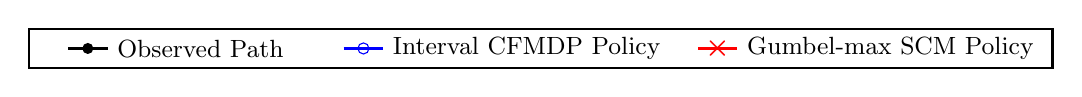
\begin{tikzpicture}[scale=1.0, every node/.style={scale=1.0}]
            \draw[thick, black] (-3, -0.25) rectangle (10, 0.25);
            %
            \draw[black, line width=1pt] (-2.5, 0.0) -- (-2,0.0);
            \fill[black] (-2.25,0.0) circle (2pt); %
            \node[right] at (-2,0.0) {\small Observed Path};
            
            %
            \draw[blue, line width=1pt] (1.0,0.0) -- (1.5,0.0);
            \node[draw=blue, circle, minimum size=4pt, inner sep=0pt] at (1.25,0.0) {}; %
            \node[right] at (1.5,0.0) {\small Interval CFMDP Policy};
            
            %
            \draw[red, line width=1pt] (5.5,0) -- (6,0);
            \node[red] at (5.75,0) {$\boldsymbol{\times}$}; %
            \node[right] at (6,0) {\small Gumbel-max SCM Policy};
        \end{tikzpicture}
    }\\
    %
    \subfigure[\footnotesize Lowest cumulative reward: Interval CFMDP ($312$), Gumbel-max SCM ($312$)]{%
        \resizebox{0.76\columnwidth}{!}{
             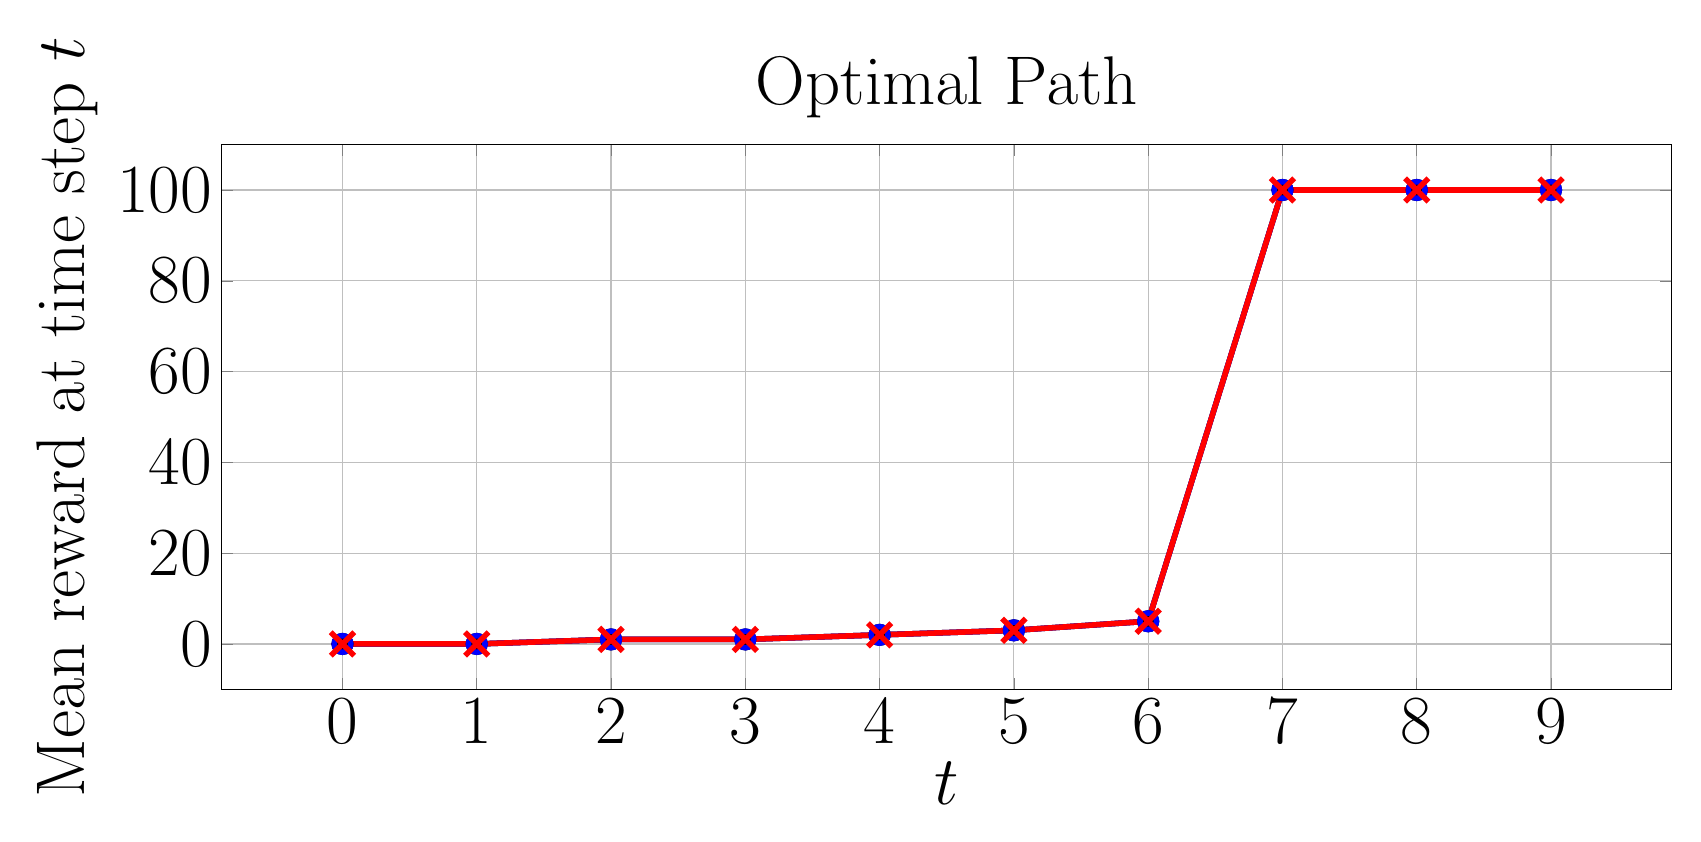
\begin{tikzpicture}
                \begin{axis}[
                    xlabel={$t$},
                    ylabel={Mean reward at time step $t$},
                    title={Optimal Path},
                    grid=both,
                    width=20cm, height=8.5cm,
                    every axis/.style={font=\Huge},
                    %
                ]
                \addplot[
                    color=black, %
                    mark=*, %
                    line width=2pt,
                    mark size=3pt,
                    error bars/.cd,
                    y dir=both, %
                    y explicit, %
                    error bar style={line width=1pt,solid},
                    error mark options={line width=1pt,mark size=4pt,rotate=90}
                ]
                coordinates {
                    (0, 0.0)  +- (0, 0.0)
                    (1, 0.0)  +- (0, 0.0) 
                    (2, 1.0)  +- (0, 0.0) 
                    (3, 1.0)  +- (0, 0.0)
                    (4, 2.0)  +- (0, 0.0)
                    (5, 3.0) +- (0, 0.0)
                    (6, 5.0) +- (0, 0.0)
                    (7, 100.0) +- (0, 0.0)
                    (8, 100.0) +- (0, 0.0)
                    (9, 100.0) +- (0, 0.0)
                };
                %
                \addplot[
                    color=blue, %
                    mark=o, %
                    line width=2pt,
                    mark size=3pt,
                    error bars/.cd,
                    y dir=both, %
                    y explicit, %
                    error bar style={line width=1pt,solid},
                    error mark options={line width=1pt,mark size=4pt,rotate=90}
                ]
                 coordinates {
                    (0, 0.0)  +- (0, 0.0)
                    (1, 0.0)  +- (0, 0.0) 
                    (2, 1.0)  +- (0, 0.0) 
                    (3, 1.0)  +- (0, 0.0)
                    (4, 2.0)  +- (0, 0.0)
                    (5, 3.0) +- (0, 0.0)
                    (6, 5.0) +- (0, 0.0)
                    (7, 100.0) +- (0, 0.0)
                    (8, 100.0) +- (0, 0.0)
                    (9, 100.0) +- (0, 0.0)
                };
                %
                \addplot[
                    color=red, %
                    mark=x, %
                    line width=2pt,
                    mark size=6pt,
                    error bars/.cd,
                    y dir=both, %
                    y explicit, %
                    error bar style={line width=1pt,solid},
                    error mark options={line width=1pt,mark size=4pt,rotate=90}
                ]
                coordinates {
                    (0, 0.0)  +- (0, 0.0)
                    (1, 0.0)  +- (0, 0.0) 
                    (2, 1.0)  +- (0, 0.0) 
                    (3, 1.0)  +- (0, 0.0)
                    (4, 2.0)  +- (0, 0.0)
                    (5, 3.0) +- (0, 0.0)
                    (6, 5.0) +- (0, 0.0)
                    (7, 100.0) +- (0, 0.0)
                    (8, 100.0) +- (0, 0.0)
                    (9, 100.0) +- (0, 0.0)
                };
                \end{axis}
            \end{tikzpicture}
         }
    }
    \hspace{1cm}
    \subfigure[\footnotesize Lowest cumulative reward: Interval CFMDP ($19$), Gumbel-max SCM ($-88$)]{%
         \resizebox{0.76\columnwidth}{!}{
            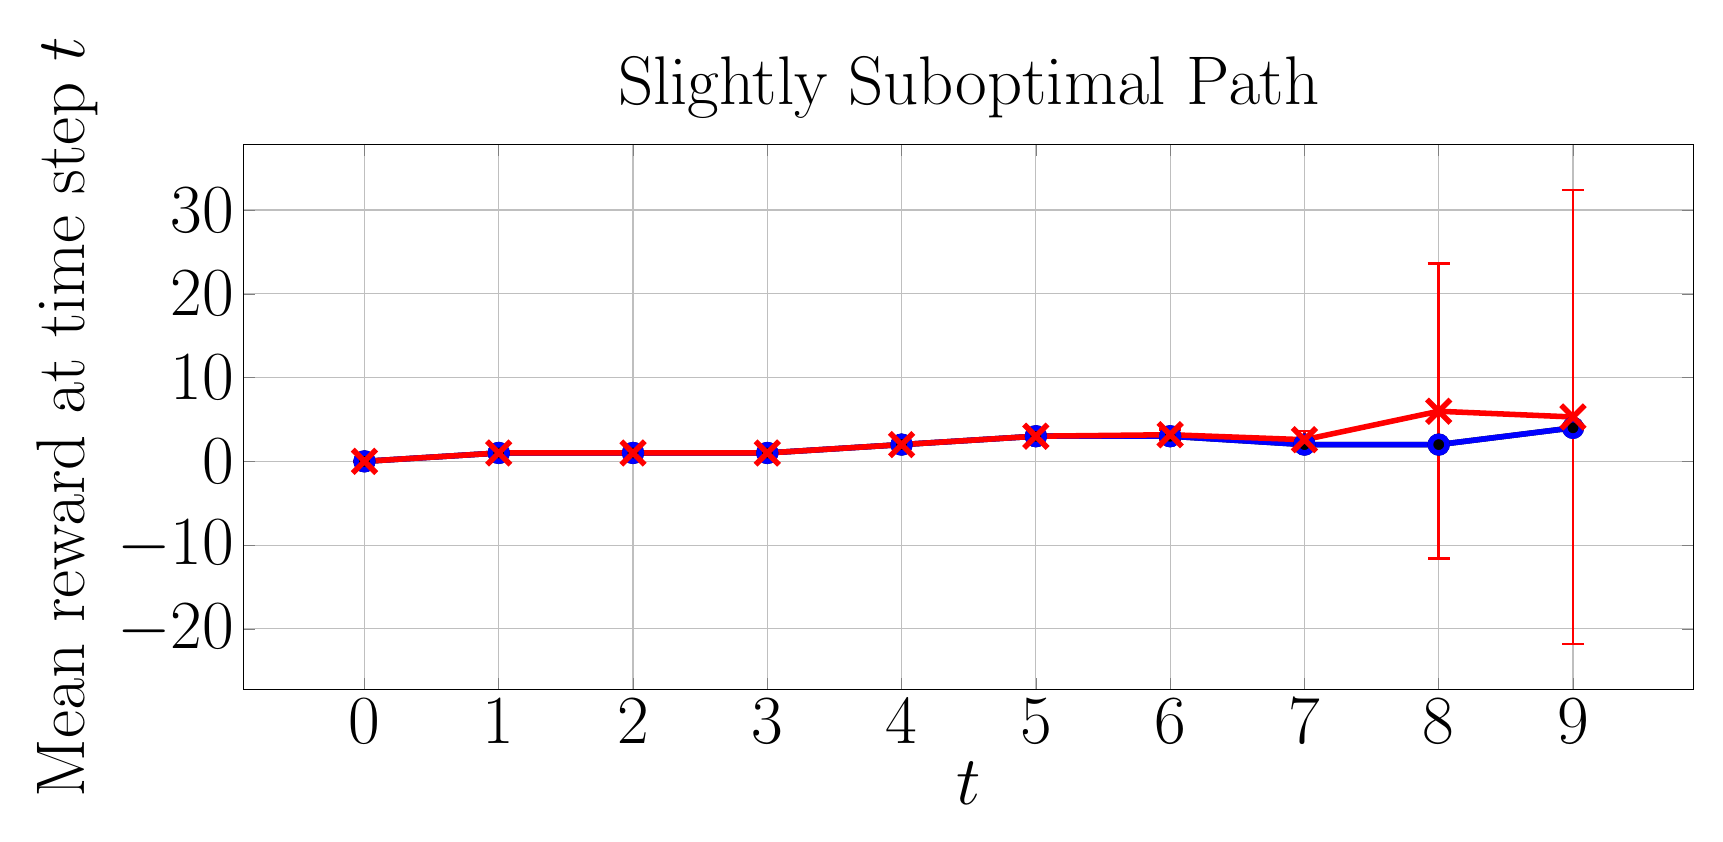
\begin{tikzpicture}
                \begin{axis}[
                    xlabel={$t$},
                    ylabel={Mean reward at time step $t$},
                    title={Slightly Suboptimal Path},
                    grid=both,
                    width=20cm, height=8.5cm,
                    every axis/.style={font=\Huge},
                    %
                ]
                \addplot[
                    color=black, %
                    mark=*, %
                    line width=2pt,
                    mark size=3pt,
                    error bars/.cd,
                    y dir=both, %
                    y explicit, %
                    error bar style={line width=1pt,solid},
                    error mark options={line width=1pt,mark size=4pt,rotate=90}
                ]
              coordinates {
                    (0, 0.0)  +- (0, 0.0)
                    (1, 1.0)  +- (0, 0.0) 
                    (2, 1.0)  +- (0, 0.0) 
                    (3, 1.0)  +- (0, 0.0)
                    (4, 2.0)  +- (0, 0.0)
                    (5, 3.0) +- (0, 0.0)
                    (6, 3.0) +- (0, 0.0)
                    (7, 2.0) +- (0, 0.0)
                    (8, 2.0) +- (0, 0.0)
                    (9, 4.0) +- (0, 0.0)
                };
                %
                \addplot[
                    color=blue, %
                    mark=o, %
                    line width=2pt,
                    mark size=3pt,
                    error bars/.cd,
                    y dir=both, %
                    y explicit, %
                    error bar style={line width=1pt,solid},
                    error mark options={line width=1pt,mark size=4pt,rotate=90}
                ]
              coordinates {
                    (0, 0.0)  +- (0, 0.0)
                    (1, 1.0)  +- (0, 0.0) 
                    (2, 1.0)  +- (0, 0.0) 
                    (3, 1.0)  +- (0, 0.0)
                    (4, 2.0)  +- (0, 0.0)
                    (5, 3.0) +- (0, 0.0)
                    (6, 3.0) +- (0, 0.0)
                    (7, 2.0) +- (0, 0.0)
                    (8, 2.0) +- (0, 0.0)
                    (9, 4.0) +- (0, 0.0)
                };
                %
                \addplot[
                    color=red, %
                    mark=x, %
                    line width=2pt,
                    mark size=6pt,
                    error bars/.cd,
                    y dir=both, %
                    y explicit, %
                    error bar style={line width=1pt,solid},
                    error mark options={line width=1pt,mark size=4pt,rotate=90}
                ]
                coordinates {
                    (0, 0.0)  +- (0, 0.0)
                    (1, 1.0)  +- (0, 0.0) 
                    (2, 1.0)  +- (0, 0.0) 
                    (3, 1.0)  +- (0, 0.0)
                    (4, 2.0)  += (0, 0.0)
                    (5, 3.0)  += (0, 0.0)
                    (6, 3.17847) += (0, 0.62606746) -= (0, 0.62606746)
                    (7, 2.5832885) += (0, 1.04598233) -= (0, 1.04598233)
                    (8, 5.978909) += (0, 17.60137623) -= (0, 17.60137623)
                    (9, 5.297059) += (0, 27.09227512) -= (0, 27.09227512)
                };
                \end{axis}
            \end{tikzpicture}
         }
    }\\[-1.5pt]
    \subfigure[\footnotesize Lowest cumulative reward: Interval CFMDP ($14$), Gumbel-max SCM ($-598$)]{%
         \resizebox{0.76\columnwidth}{!}{
             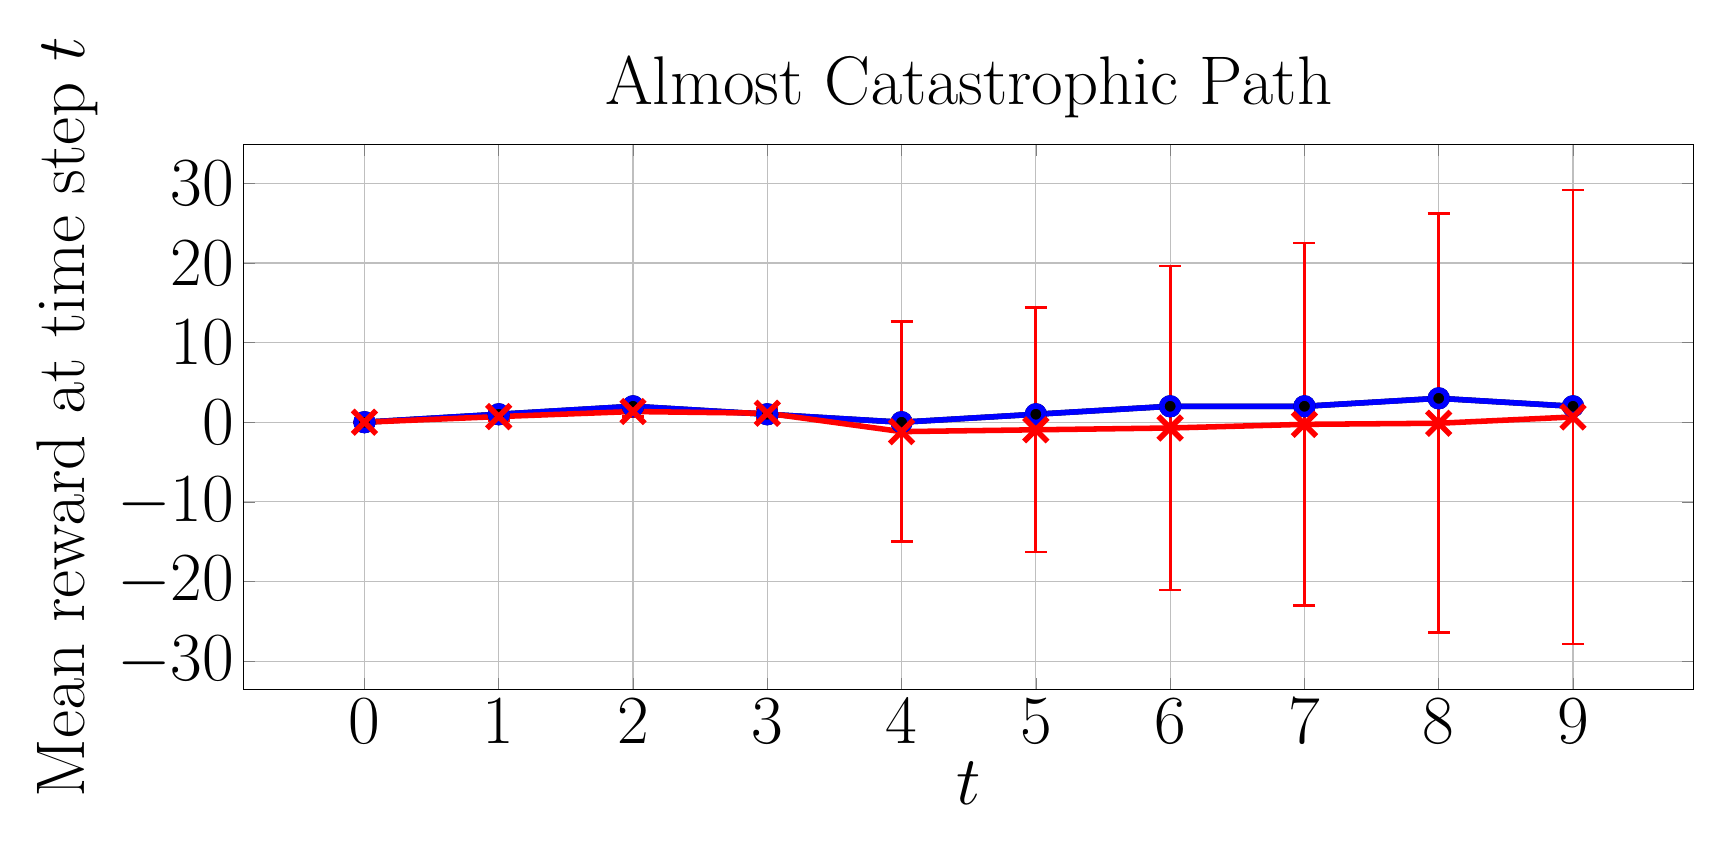
\begin{tikzpicture}
                \begin{axis}[
                    xlabel={$t$},
                    ylabel={Mean reward at time step $t$},
                    title={Almost Catastrophic Path},
                    grid=both,
                    width=20cm, height=8.5cm,
                    every axis/.style={font=\Huge},
                    %
                ]
                \addplot[
                    color=black, %
                    mark=*, %
                    line width=2pt,
                    mark size=3pt,
                    error bars/.cd,
                    y dir=both, %
                    y explicit, %
                    error bar style={line width=1pt,solid},
                    error mark options={line width=1pt,mark size=4pt,rotate=90}
                ]
                coordinates {
                    (0, 0.0)  +- (0, 0.0)
                    (1, 1.0)  +- (0, 0.0) 
                    (2, 2.0)  +- (0, 0.0) 
                    (3, 1.0)  +- (0, 0.0)
                    (4, 0.0)  +- (0, 0.0)
                    (5, 1.0) +- (0, 0.0)
                    (6, 2.0) +- (0, 0.0)
                    (7, 2.0) +- (0, 0.0)
                    (8, 3.0) +- (0, 0.0)
                    (9, 2.0) +- (0, 0.0)
                };
                %
                \addplot[
                    color=blue, %
                    mark=o, %
                    line width=2pt,
                    mark size=3pt,
                    error bars/.cd,
                    y dir=both, %
                    y explicit, %
                    error bar style={line width=1pt,solid},
                    error mark options={line width=1pt,mark size=4pt,rotate=90}
                ]
                coordinates {
                    (0, 0.0)  +- (0, 0.0)
                    (1, 1.0)  +- (0, 0.0) 
                    (2, 2.0)  +- (0, 0.0) 
                    (3, 1.0)  +- (0, 0.0)
                    (4, 0.0)  +- (0, 0.0)
                    (5, 1.0) +- (0, 0.0)
                    (6, 2.0) +- (0, 0.0)
                    (7, 2.0) +- (0, 0.0)
                    (8, 3.0) +- (0, 0.0)
                    (9, 2.0) +- (0, 0.0)
                };
                %
                \addplot[
                    color=red, %
                    mark=x, %
                    line width=2pt,
                    mark size=6pt,
                    error bars/.cd,
                    y dir=both, %
                    y explicit, %
                    error bar style={line width=1pt,solid},
                    error mark options={line width=1pt,mark size=4pt,rotate=90}
                ]
                coordinates {
                    (0, 0.0)  +- (0, 0.0)
                    (1, 0.7065655)  +- (0, 0.4553358) 
                    (2, 1.341673)  +- (0, 0.67091621) 
                    (3, 1.122926)  +- (0, 0.61281824)
                    (4, -1.1821935)  +- (0, 13.82444042)
                    (5, -0.952399)  +- (0, 15.35195457)
                    (6, -0.72672) +- (0, 20.33508414)
                    (7, -0.268983) +- (0, 22.77861454)
                    (8, -0.1310835) +- (0, 26.31013314)
                    (9, 0.65806) +- (0, 28.50670214)
                };
                %
            %
            %
            %
            %
            %
            %
            %
            %
            %
            %
            %
            %
            %
            %
            %
            %
            %
            %
                \end{axis}
            \end{tikzpicture}
         }
    }
    \hspace{1cm}
    \subfigure[\footnotesize Lowest cumulative reward: Interval CFMDP ($-698$), Gumbel-max SCM ($-698$)]{%
         \resizebox{0.76\columnwidth}{!}{
            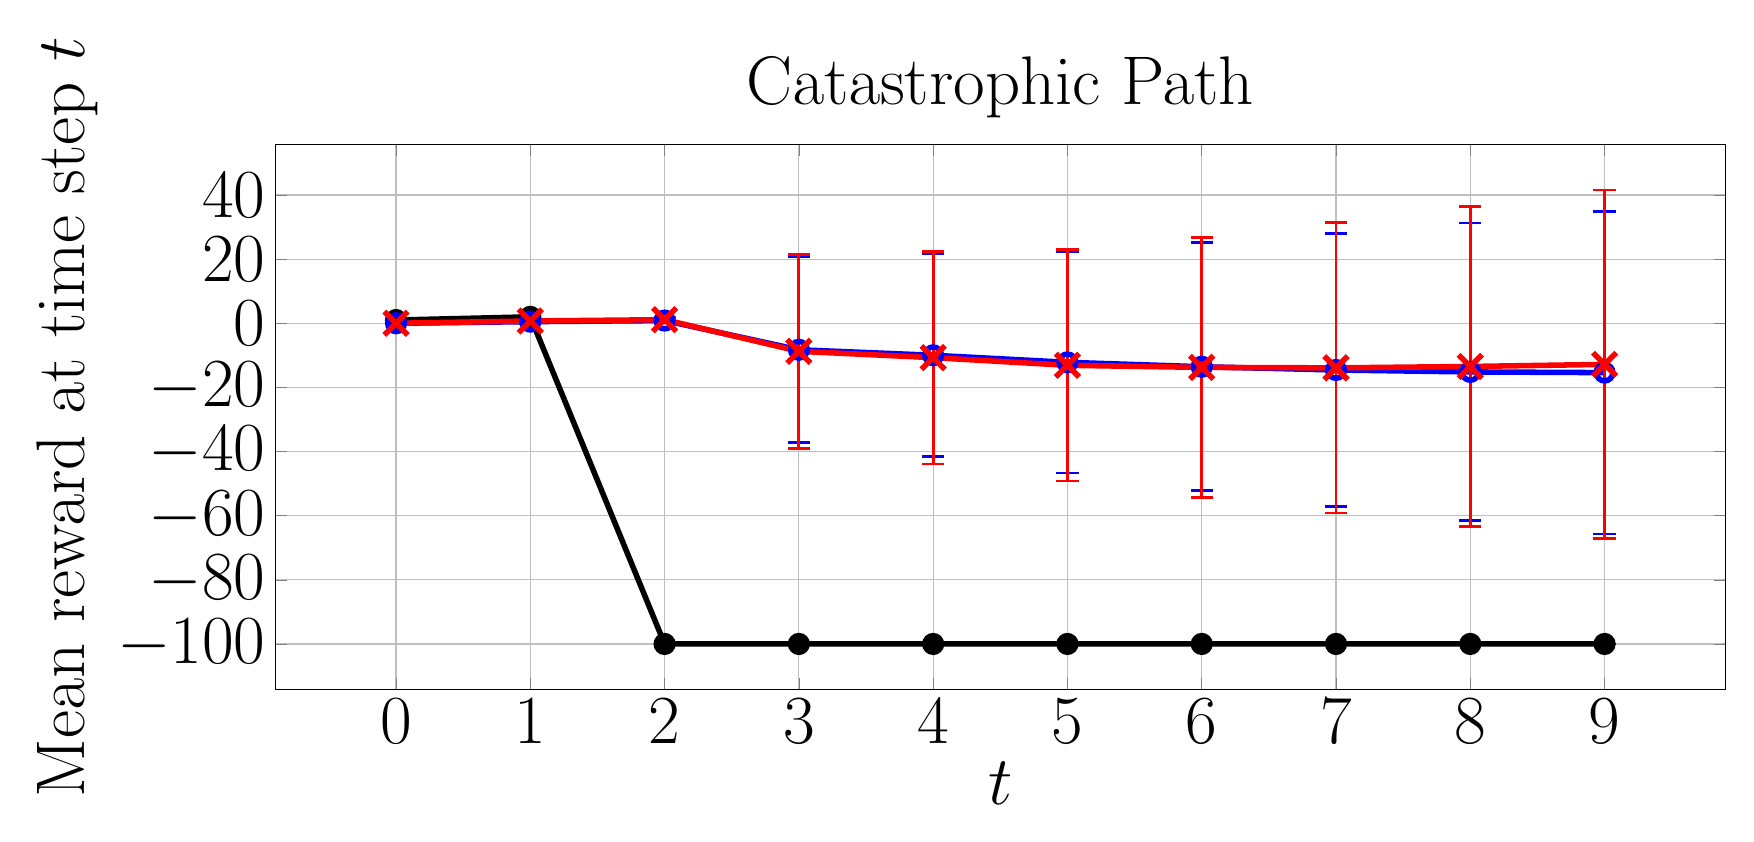
\begin{tikzpicture}
                \begin{axis}[
                    xlabel={$t$},
                    ylabel={Mean reward at time step $t$},
                    title={Catastrophic Path},
                    grid=both,
                    width=20cm, height=8.5cm,
                    every axis/.style={font=\Huge},
                    %
                ]
                \addplot[
                    color=black, %
                    mark=*, %
                    line width=2pt,
                    mark size=3pt,
                    error bars/.cd,
                    y dir=both, %
                    y explicit, %
                    error bar style={line width=1pt,solid},
                    error mark options={line width=1pt,mark size=4pt,rotate=90}
                ]
                coordinates {
                    (0, 1.0)  +- (0, 0.0)
                    (1, 2.0)  +- (0, 0.0) 
                    (2, -100.0)  +- (0, 0.0) 
                    (3, -100.0)  +- (0, 0.0)
                    (4, -100.0)  +- (0, 0.0)
                    (5, -100.0) +- (0, 0.0)
                    (6, -100.0) +- (0, 0.0)
                    (7, -100.0) +- (0, 0.0)
                    (8, -100.0) +- (0, 0.0)
                    (9, -100.0) +- (0, 0.0)
                };
                %
                \addplot[
                    color=blue, %
                    mark=o, %
                    line width=2pt,
                    mark size=3pt,
                    error bars/.cd,
                    y dir=both, %
                    y explicit, %
                    error bar style={line width=1pt,solid},
                    error mark options={line width=1pt,mark size=4pt,rotate=90}
                ]
                coordinates {
                    (0, 0.0)  +- (0, 0.0)
                    (1, 0.504814)  +- (0, 0.49997682) 
                    (2, 0.8439835)  +- (0, 0.76831917) 
                    (3, -8.2709165)  +- (0, 28.93656754)
                    (4, -9.981082)  +- (0, 31.66825363)
                    (5, -12.1776325) +- (0, 34.53463233)
                    (6, -13.556076) +- (0, 38.62845372)
                    (7, -14.574418) +- (0, 42.49603359)
                    (8, -15.1757075) +- (0, 46.41913968)
                    (9, -15.3900395) +- (0, 50.33563368)
                };
                %
                \addplot[
                    color=red, %
                    mark=x, %
                    line width=2pt,
                    mark size=6pt,
                    error bars/.cd,
                    y dir=both, %
                    y explicit, %
                    error bar style={line width=1pt,solid},
                    error mark options={line width=1pt,mark size=4pt,rotate=90}
                ]
                coordinates {
                    (0, 0.0)  +- (0, 0.0)
                    (1, 0.701873)  +- (0, 0.45743556) 
                    (2, 1.1227805)  +- (0, 0.73433129) 
                    (3, -8.7503255)  +- (0, 30.30257976)
                    (4, -10.722092)  +- (0, 33.17618589)
                    (5, -13.10721)  +- (0, 36.0648089)
                    (6, -13.7631645) +- (0, 40.56553451)
                    (7, -13.909043) +- (0, 45.23829402)
                    (8, -13.472517) +- (0, 49.96270296)
                    (9, -12.8278835) +- (0, 54.38618735)
                };
                %
            %
            %
            %
            %
            %
            %
            %
            %
            %
            %
            %
            %
            %
            %
            %
            %
            %
            %
                \end{axis}
            \end{tikzpicture}
         }
    }
    \caption{Average instant reward of CF paths induced by policies on GridWorld $p=0.4$.}
    \label{fig: reward p=0.4}
\end{figure*}

\subsection{Experimental Setup}
To compare policy performance, we measure the average rewards of counterfactual paths induced by our policy and the Gumbel-max policy by uniformly sampling $200$ counterfactual MDPs from the ICFMDP and generating $10,000$ counterfactual paths over each sampled CFMDP. \jl{Since the interval CFMDP depends on the observed path, we select $4$  paths of varying optimality to evaluate how the observed path impacts the performance of both policies: an optimal path, a slightly suboptimal path that could reach the optimal reward with a few changes, a catastrophic path that enters a catastrophic, terminal state with low reward, and an almost catastrophic path that was close to entering a catastrophic state.} When measuring the average probability bound widths and execution time needed to generate the ICFMDPs, we averaged over $20$ randomly generated observed paths
\footnote{Further training details are provided in Appendix \ref{app: training details}, and the code is provided at \href{https://github.com/ddv-lab/robust-cf-inference-in-MDPs}{https://github.com/ddv-lab/robust-cf-inference-in-MDPs}
%
%
.}.

\subsection{GridWorld}
\jl{The GridWorld MDP is a $4 \times 4$ grid where an agent must navigate from the top-left corner to the goal state in the bottom-right corner, avoiding a dangerous terminal state in the centre. At each time step, the agent can move up, down, left, or right, but there is a small probability (controlled by hyper-parameter $p$) of moving in an unintended direction. As the agent nears the goal, the reward for each state increases, culminating in a reward of $+100$ for reaching the goal. Entering the dangerous state results in a penalty of $-100$. We use two versions of GridWorld: a less stochastic version with $p=0.9$ (i.e., $90$\% chance of moving in the chosen direction) and a more stochastic version with $p=0.4$.}

\paragraph{GridWorld ($p=0.9$)}
When $p=0.9$, the counterfactual probability bounds are typically narrow (see Table \ref{tab:nonzero_probs} for average measurements). Consequently, as shown in Figure \ref{fig: reward p=0.9}, both policies are nearly identical and perform similarly well across the optimal, slightly suboptimal, and catastrophic paths.
%
However, for the almost catastrophic path, the interval CFMDP path is more conservative and follows the observed path more closely (as this is where the probability bounds are narrowest), which typically requires one additional step to reach the goal state than the Gumbel-max SCM policy.
%

\paragraph{GridWorld ($p=0.4$)}
\jl{When $p=0.4$, the GridWorld environment becomes more uncertain, increasing the risk of entering the dangerous state even if correct actions are chosen. Thus, as shown in Figure \ref{fig: reward p=0.4}, the interval CFMDP policy adopts a more conservative approach, avoiding deviation from the observed policy if it cannot guarantee higher counterfactual rewards (see the slightly suboptimal and almost catastrophic paths), whereas the Gumbel-max SCM is inconsistent: it can yield higher rewards, but also much lower rewards, reflected in the wide error bars.} For the catastrophic path, both policies must deviate from the observed path to achieve a higher reward and, in this case, perform similarly.
%
%
%
%
\subsection{Sepsis}
The Sepsis MDP \citep{oberst2019counterfactual} simulates trajectories of Sepsis patients. Each state consists of four vital signs (heart rate, blood pressure, oxygen concentration, and glucose levels), categorised as low, normal, or high.
and three treatments that can be toggled on/off at each time step (8 actions in total). Unlike \citet{oberst2019counterfactual}, we scale rewards based on the number of out-of-range vital signs, between $-1000$ (patient dies) and $1000$ (patient discharged). \jl{Like the GridWorld $p=0.4$ experiment, the Sepsis MDP is highly uncertain, as many states are equally likely to lead to optimal and poor outcomes. Thus, as shown in Figure \ref{fig: reward sepsis}, both policies follow the observed optimal and almost catastrophic paths to guarantee rewards are no worse than the observation.} However, improving the catastrophic path requires deviating from the observation. Here, the Gumbel-max SCM policy, on average, performs better than the interval CFMDP policy. But, since both policies have lower bounds clipped at $-1000$, neither policy reliably improves over the observation. In contrast, for the slightly suboptimal path, the interval CFMDP policy performs significantly better, shown by its higher lower bounds. 
Moreover, in these two cases, the worst-case counterfactual path generated by the interval CFMDP policy is better than that of the Gumbel-max SCM policy,
indicating its greater robustness.
%
\begin{figure*}
    \centering
     \resizebox{0.6\textwidth}{!}{
        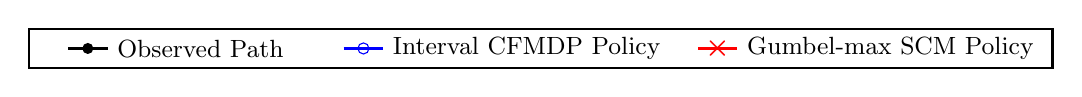
\begin{tikzpicture}[scale=1.0, every node/.style={scale=1.0}]
            \draw[thick, black] (-3, -0.25) rectangle (10, 0.25);
            %
            \draw[black, line width=1pt] (-2.5, 0.0) -- (-2,0.0);
            \fill[black] (-2.25,0.0) circle (2pt); %
            \node[right] at (-2,0.0) {\small Observed Path};
            
            %
            \draw[blue, line width=1pt] (1.0,0.0) -- (1.5,0.0);
            \node[draw=blue, circle, minimum size=4pt, inner sep=0pt] at (1.25,0.0) {}; %
            \node[right] at (1.5,0.0) {\small Interval CFMDP Policy};
            
            %
            \draw[red, line width=1pt] (5.5,0) -- (6,0);
            \node[red] at (5.75,0) {$\boldsymbol{\times}$}; %
            \node[right] at (6,0) {\small Gumbel-max SCM Policy};
        \end{tikzpicture}
    }\\
    \subfigure[\footnotesize Lowest cumulative reward: Interval CFMDP ($8000$), Gumbel-max SCM ($8000$)]{%
         \resizebox{0.76\columnwidth}{!}{
             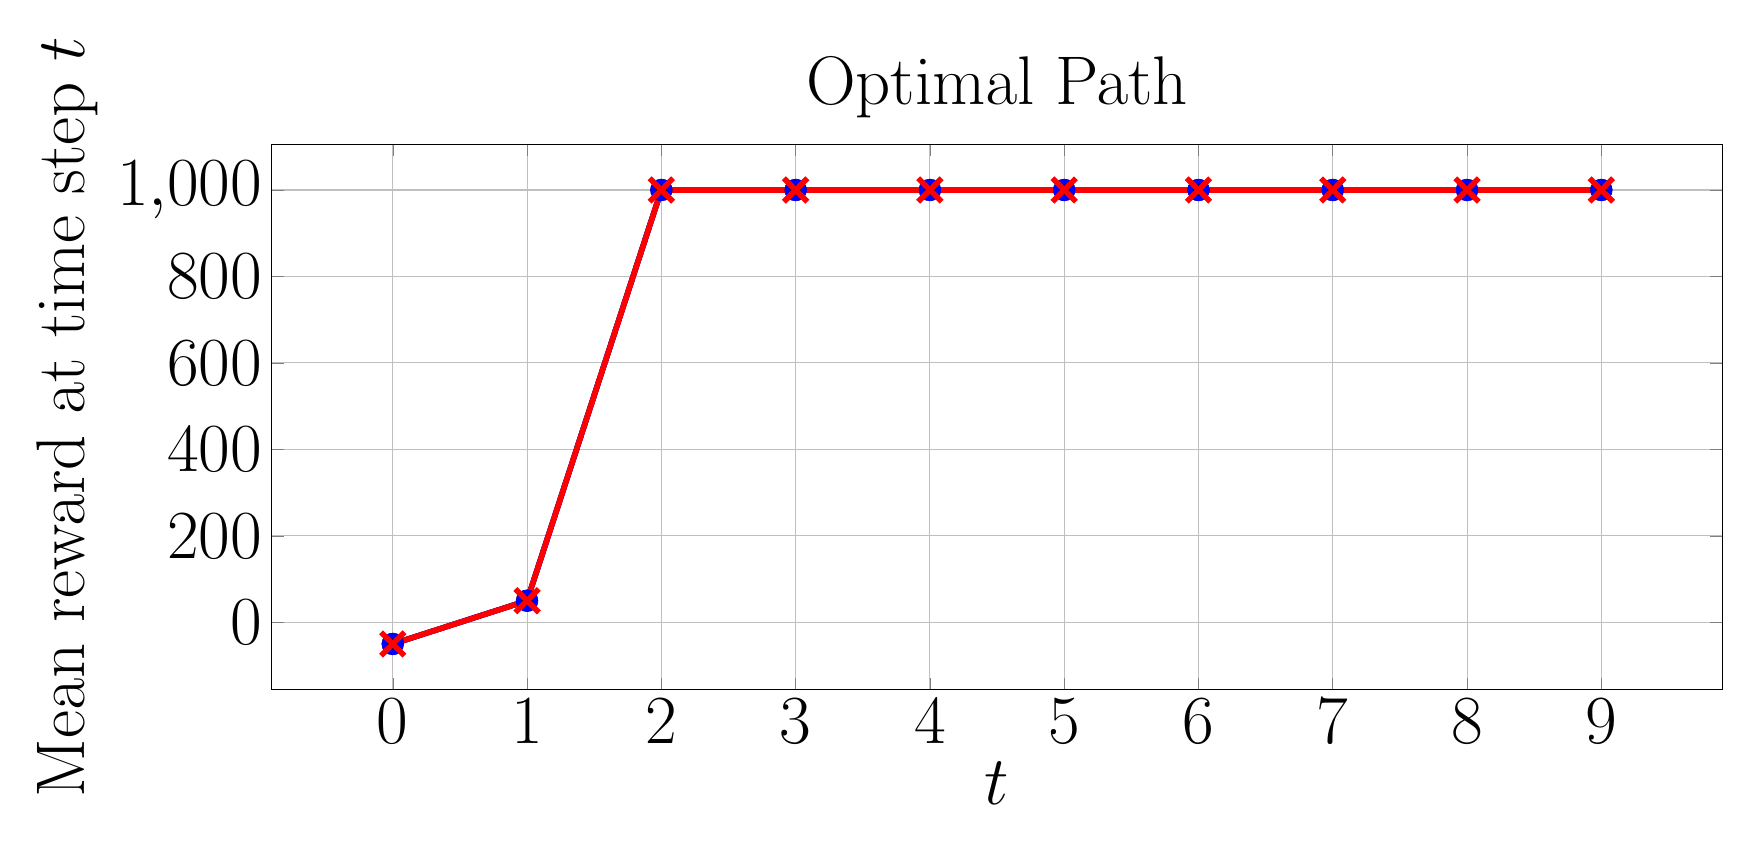
\begin{tikzpicture}
                \begin{axis}[
                    xlabel={$t$},
                    ylabel={Mean reward at time step $t$},
                    title={Optimal Path},
                    grid=both,
                    width=20cm, height=8.5cm,
                    every axis/.style={font=\Huge},
                    %
                ]
                \addplot[
                    color=black, %
                    mark=*, %
                    line width=2pt,
                    mark size=3pt,
                ]
                coordinates {
                    (0, -50.0)
                    (1, 50.0)
                    (2, 1000.0)
                    (3, 1000.0)
                    (4, 1000.0)
                    (5, 1000.0)
                    (6, 1000.0)
                    (7, 1000.0)
                    (8, 1000.0)
                    (9, 1000.0)
                };
                %
                \addplot[
                    color=blue, %
                    mark=o, %
                    line width=2pt,
                    mark size=3pt,
                    error bars/.cd,
                    y dir=both, %
                    y explicit, %
                    error bar style={line width=1pt,solid},
                    error mark options={line width=1pt,mark size=4pt,rotate=90}
                ]
                coordinates {
                    (0, -50.0)  +- (0, 0.0)
                    (1, 50.0)  +- (0, 0.0) 
                    (2, 1000.0)  +- (0, 0.0) 
                    (3, 1000.0)  +- (0, 0.0)
                    (4, 1000.0)  +- (0, 0.0)
                    (5, 1000.0) +- (0, 0.0)
                    (6, 1000.0) +- (0, 0.0)
                    (7, 1000.0) +- (0, 0.0)
                    (8, 1000.0) +- (0, 0.0)
                    (9, 1000.0) +- (0, 0.0)
                };
                %
                \addplot[
                    color=red, %
                    mark=x, %
                    line width=2pt,
                    mark size=6pt,
                    error bars/.cd,
                    y dir=both, %
                    y explicit, %
                    error bar style={line width=1pt,solid},
                    error mark options={line width=1pt,mark size=4pt,rotate=90}
                ]
                coordinates {
                    (0, -50.0)  +- (0, 0.0)
                    (1, 50.0)  +- (0, 0.0) 
                    (2, 1000.0)  +- (0, 0.0) 
                    (3, 1000.0)  +- (0, 0.0)
                    (4, 1000.0)  +- (0, 0.0)
                    (5, 1000.0) +- (0, 0.0)
                    (6, 1000.0) +- (0, 0.0)
                    (7, 1000.0) +- (0, 0.0)
                    (8, 1000.0) +- (0, 0.0)
                    (9, 1000.0) +- (0, 0.0)
                };
                %
                \end{axis}
            \end{tikzpicture}
         }
    }
    \hspace{1cm}
    \subfigure[\footnotesize Lowest cumulative reward: Interval CFMDP ($-5980$), Gumbel-max SCM ($-8000$)]{%
         \resizebox{0.76\columnwidth}{!}{
            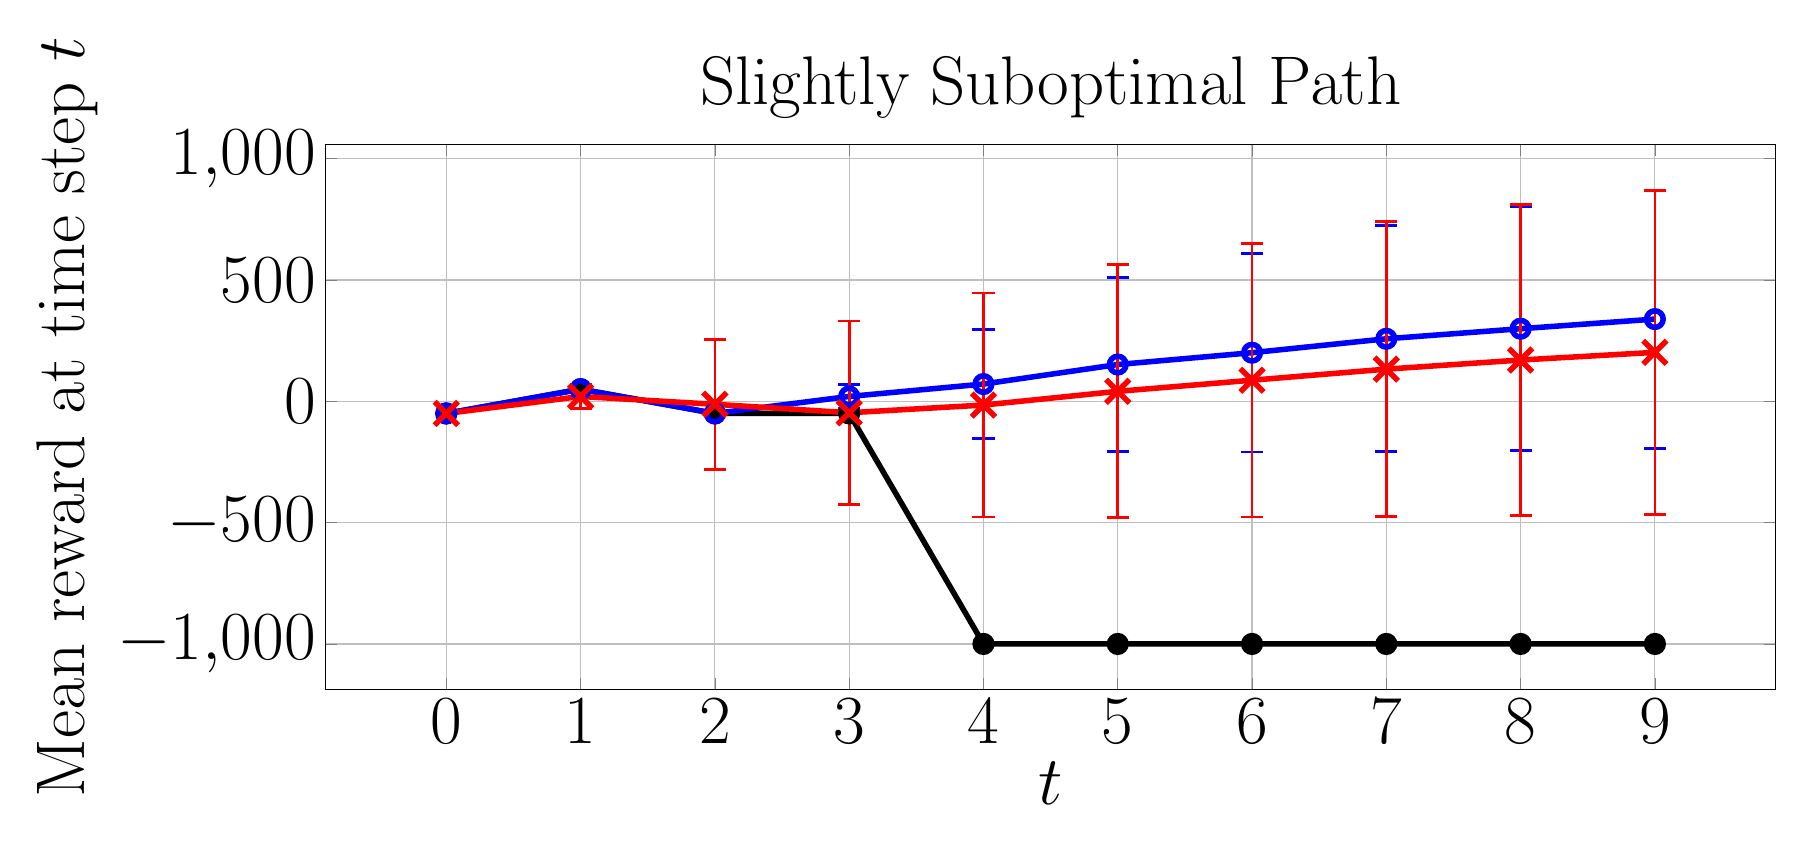
\begin{tikzpicture}
                \begin{axis}[
                    xlabel={$t$},
                    ylabel={Mean reward at time step $t$},
                    title={Slightly Suboptimal Path},
                    grid=both,
                    width=20cm, height=8.5cm,
                    every axis/.style={font=\Huge},
                    %
                ]
               \addplot[
                    color=black, %
                    mark=*, %
                    line width=2pt,
                    mark size=3pt,
                ]
                coordinates {
                    (0, -50.0)
                    (1, 50.0)
                    (2, -50.0)
                    (3, -50.0)
                    (4, -1000.0)
                    (5, -1000.0)
                    (6, -1000.0)
                    (7, -1000.0)
                    (8, -1000.0)
                    (9, -1000.0)
                };
                %
                \addplot[
                    color=blue, %
                    mark=o, %
                    line width=2pt,
                    mark size=3pt,
                    error bars/.cd,
                    y dir=both, %
                    y explicit, %
                    error bar style={line width=1pt,solid},
                    error mark options={line width=1pt,mark size=4pt,rotate=90}
                ]
                coordinates {
                    (0, -50.0)  +- (0, 0.0)
                    (1, 50.0)  +- (0, 0.0) 
                    (2, -50.0)  +- (0, 0.0) 
                    (3, 20.0631)  +- (0, 49.97539413)
                    (4, 71.206585)  +- (0, 226.02033693)
                    (5, 151.60797) +- (0, 359.23292559)
                    (6, 200.40593) +- (0, 408.86185176)
                    (7, 257.77948) +- (0, 466.10372804)
                    (8, 299.237465) +- (0, 501.82579506)
                    (9, 338.9129) +- (0, 532.06124996)
                };
                %
                \addplot[
                    color=red, %
                    mark=x, %
                    line width=2pt,
                    mark size=6pt,
                    error bars/.cd,
                    y dir=both, %
                    y explicit, %
                    error bar style={line width=1pt,solid},
                    error mark options={line width=1pt,mark size=4pt,rotate=90}
                ]
                coordinates {
                    (0, -50.0)  +- (0, 0.0)
                    (1, 20.00736)  +- (0, 49.99786741) 
                    (2, -12.282865)  +- (0, 267.598755) 
                    (3, -47.125995)  +- (0, 378.41755832)
                    (4, -15.381965)  +- (0, 461.77616558)
                    (5, 41.15459) +- (0, 521.53189262)
                    (6, 87.01595) +- (0, 564.22243126 )
                    (7, 132.62376) +- (0, 607.31338037)
                    (8, 170.168145) +- (0, 641.48013693)
                    (9, 201.813135) +- (0, 667.29441777)
                };
                %
                %
                %
                %
                %
                %
                %
                %
                %
                %
                %
                %
                %
                %
                %
                %
                %
                %
                %
                \end{axis}
            \end{tikzpicture}
         }
    }\\[-1.5pt]
    \subfigure[\footnotesize Lowest cumulative reward: Interval CFMDP ($100$), Gumbel-max SCM ($100$)]{%
         \resizebox{0.76\columnwidth}{!}{
             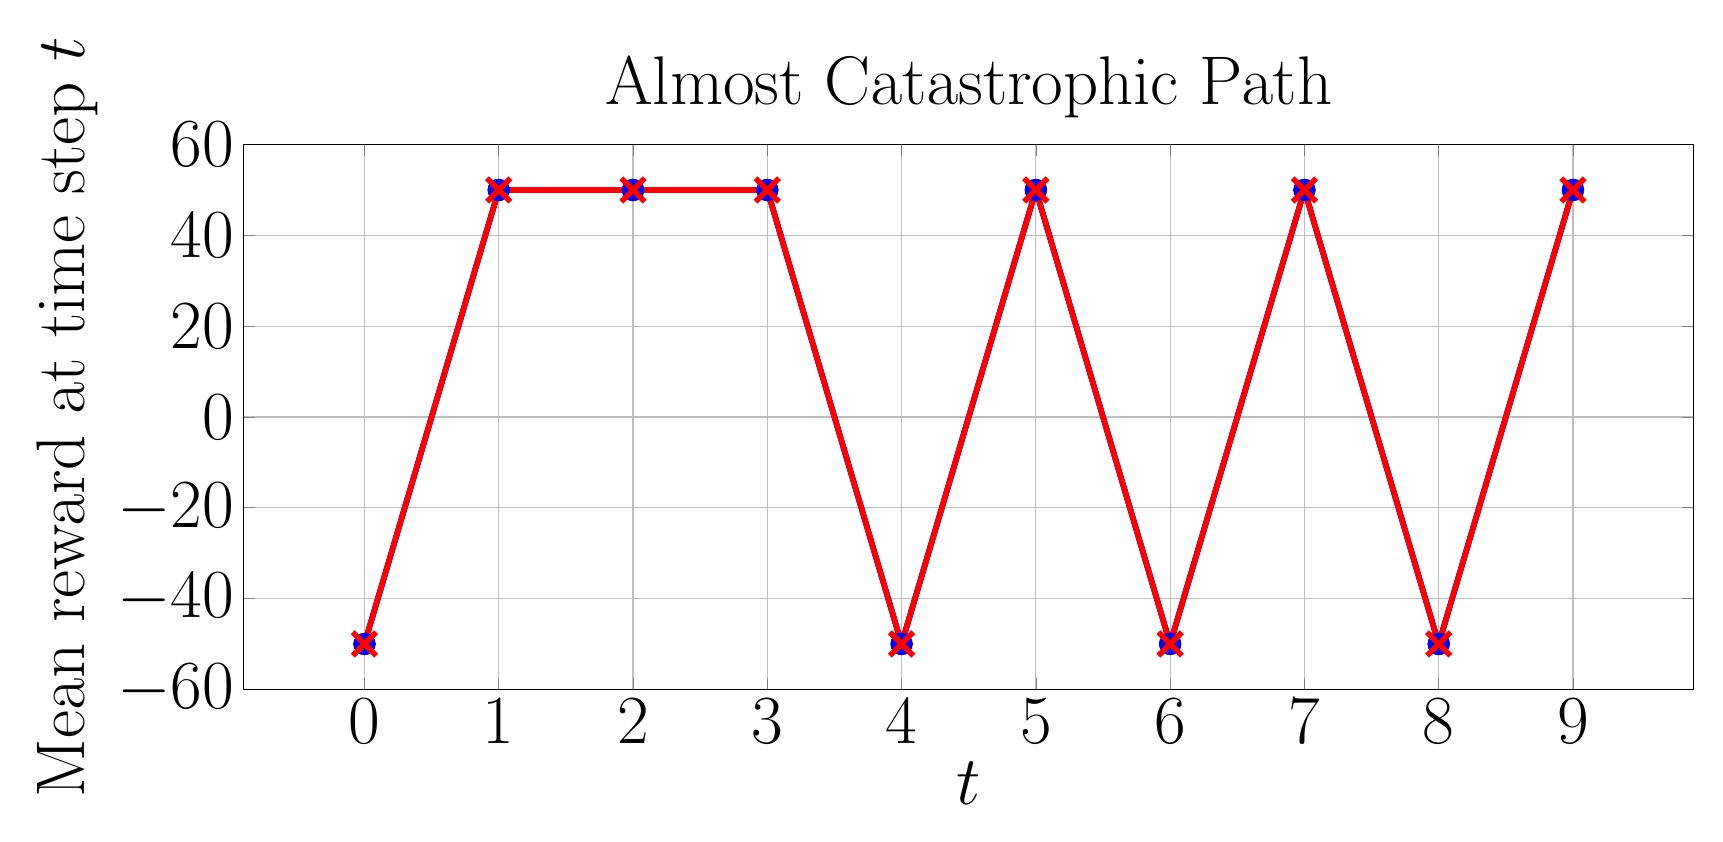
\begin{tikzpicture}
                \begin{axis}[
                    xlabel={$t$},
                    ylabel={Mean reward at time step $t$},
                    title={Almost Catastrophic Path},
                    grid=both,
                    every axis/.style={font=\Huge},
                    width=20cm, height=8.5cm,
                    %
                ]
               \addplot[
                    color=black, %
                    mark=*, %
                    line width=2pt,
                    mark size=3pt,
                ]
                coordinates {
                    (0, -50.0)
                    (1, 50.0)
                    (2, 50.0)
                    (3, 50.0)
                    (4, -50.0)
                    (5, 50.0)
                    (6, -50.0)
                    (7, 50.0)
                    (8, -50.0)
                    (9, 50.0)
                };
                %
                %
                \addplot[
                    color=blue, %
                    mark=o, %
                    line width=2pt,
                    mark size=3pt,
                    error bars/.cd,
                    y dir=both, %
                    y explicit, %
                    error bar style={line width=1pt,solid},
                    error mark options={line width=1pt,mark size=4pt,rotate=90}
                ]
                coordinates {
                    (0, -50.0)  +- (0, 0.0)
                    (1, 50.0)  +- (0, 0.0) 
                    (2, 50.0)  +- (0, 0.0) 
                    (3, 50.0)  +- (0, 0.0)
                    (4, -50.0)  +- (0, 0.0)
                    (5, 50.0) +- (0, 0.0)
                    (6, -50.0) +- (0, 0.0)
                    (7, 50.0) +- (0, 0.0)
                    (8, -50.0) +- (0, 0.0)
                    (9, 50.0) +- (0, 0.0)
                };
                %
                \addplot[
                    color=red, %
                    mark=x, %
                    line width=2pt,
                    mark size=6pt,
                    error bars/.cd,
                    y dir=both, %
                    y explicit, %
                    error bar style={line width=1pt,solid},
                    error mark options={line width=1pt,mark size=4pt,rotate=90}
                ]
                coordinates {
                    (0, -50.0)  +- (0, 0.0)
                    (1, 50.0)  +- (0, 0.0) 
                    (2, 50.0)  +- (0, 0.0) 
                    (3, 50.0)  +- (0, 0.0)
                    (4, -50.0)  +- (0, 0.0)
                    (5, 50.0) +- (0, 0.0)
                    (6, -50.0) +- (0, 0.0)
                    (7, 50.0) +- (0, 0.0)
                    (8, -50.0) +- (0, 0.0)
                    (9, 50.0) +- (0, 0.0)
                };
                %
                %
                %
                %
                %
                %
                %
                %
                %
                %
                %
                %
                %
                %
                %
                %
                %
                %
                %
                \end{axis}
            \end{tikzpicture}
         }
    }
    \hspace{1cm}
    \subfigure[\footnotesize Lowest cumulative reward: Interval CFMDP ($-7150$), Gumbel-max SCM ($-9050$)]{%
         \resizebox{0.76\columnwidth}{!}{
            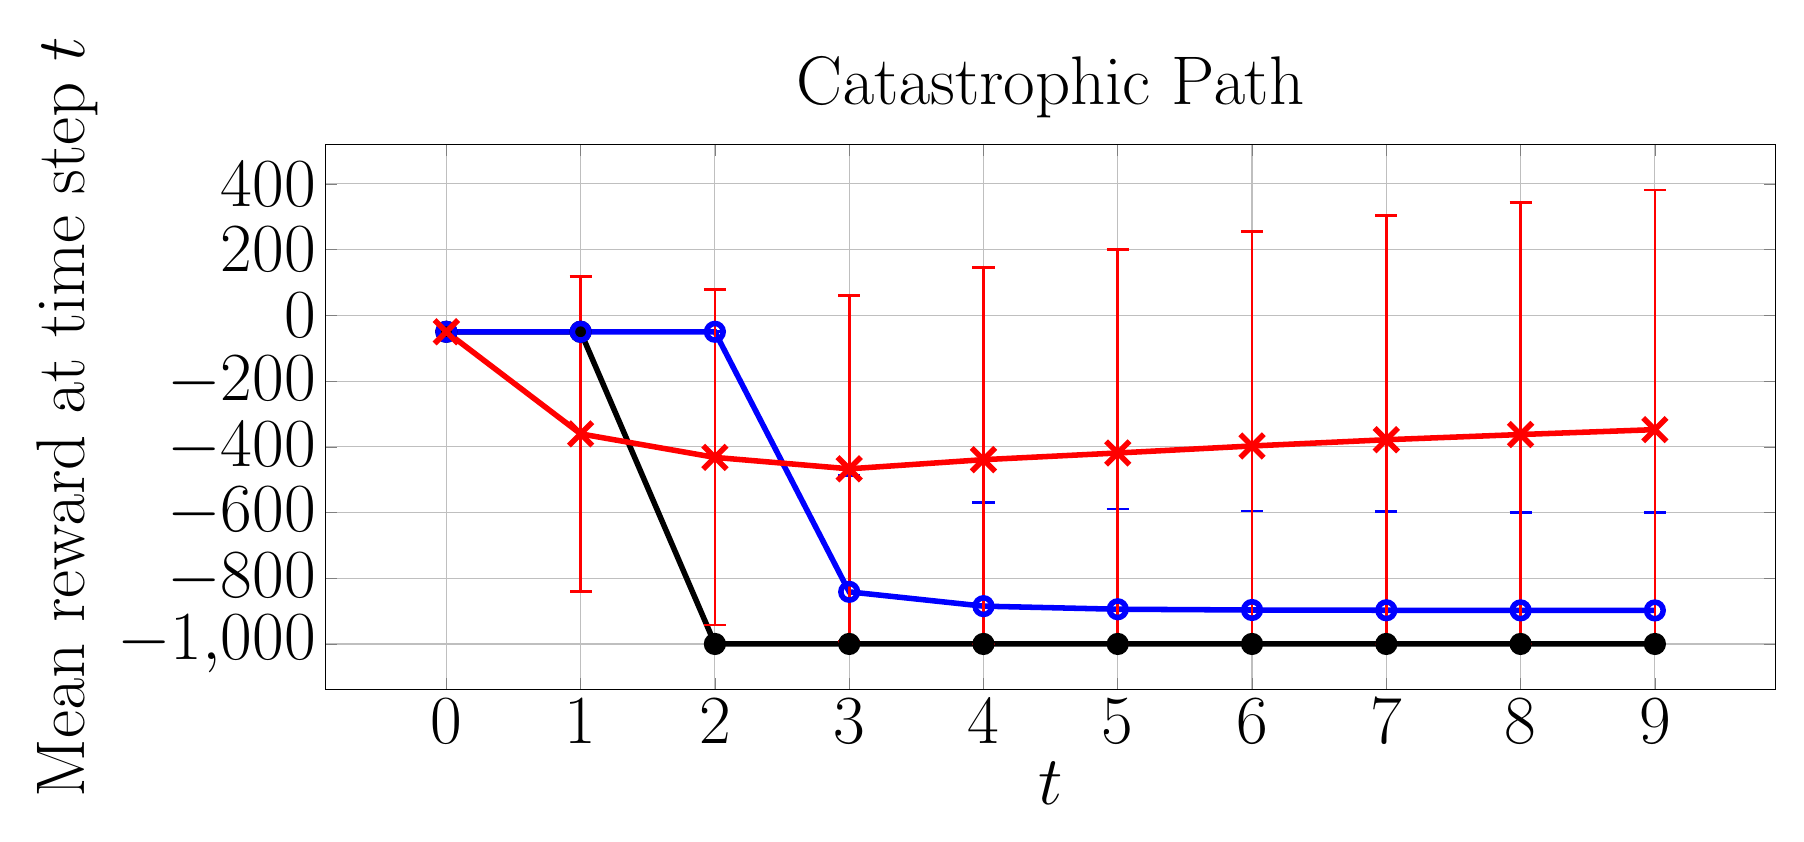
\begin{tikzpicture}
                \begin{axis}[
                    xlabel={$t$},
                    ylabel={Mean reward at time step $t$},
                    title={Catastrophic Path},
                    grid=both,
                    width=20cm, height=8.5cm,
                    every axis/.style={font=\Huge},
                    %
                ]
               \addplot[
                    color=black, %
                    mark=*, %
                    line width=2pt,
                    mark size=3pt,
                ]
                coordinates {
                    (0, -50.0)
                    (1, -50.0)
                    (2, -1000.0)
                    (3, -1000.0)
                    (4, -1000.0)
                    (5, -1000.0)
                    (6, -1000.0)
                    (7, -1000.0)
                    (8, -1000.0)
                    (9, -1000.0)
                };
                %
                %
                \addplot[
                    color=blue, %
                    mark=o, %
                    line width=2pt,
                    mark size=3pt,
                    error bars/.cd,
                    y dir=both, %
                    y explicit, %
                    error bar style={line width=1pt,solid},
                    error mark options={line width=1pt,mark size=4pt,rotate=90}
                ]
                coordinates {
                    (0, -50.0)  +- (0, 0.0)
                    (1, -50.0)  +- (0, 0.0) 
                    (2, -50.0)  +- (0, 0.0) 
                    (3, -841.440725)  += (0, 354.24605512) -= (0, 158.559275)
                    (4, -884.98225)  += (0, 315.37519669) -= (0, 115.01775)
                    (5, -894.330425) += (0, 304.88572805) -= (0, 105.669575)
                    (6, -896.696175) += (0, 301.19954514) -= (0, 103.303825)
                    (7, -897.4635) += (0, 299.61791279) -= (0, 102.5365)
                    (8, -897.77595) += (0, 298.80392585) -= (0, 102.22405)
                    (9, -897.942975) += (0, 298.32920557) -= (0, 102.057025)
                };
                %
                \addplot[
                    color=red, %
                    mark=x, %
                    line width=2pt,
                    mark size=6pt,
                    error bars/.cd,
                    y dir=both, %
                    y explicit, %
                    error bar style={line width=1pt,solid},
                    error mark options={line width=1pt,mark size=4pt,rotate=90}
                ]
            coordinates {
                    (0, -50.0)  +- (0, 0.0)
                    (1, -360.675265)  +- (0, 479.39812699) 
                    (2, -432.27629)  +- (0, 510.38620897) 
                    (3, -467.029545)  += (0, 526.36009628) -= (0, 526.36009628)
                    (4, -439.17429)  += (0, 583.96638919) -= (0, 560.82571)
                    (5, -418.82704) += (0, 618.43027478) -= (0, 581.17296)
                    (6, -397.464895) += (0, 652.67322574) -= (0, 602.535105)
                    (7, -378.49052) += (0, 682.85407033) -= (0, 621.50948)
                    (8, -362.654195) += (0, 707.01412023) -= (0, 637.345805)
                    (9, -347.737935) += (0, 729.29076479) -= (0, 652.262065)
                };
                %
                %
                %
                %
                %
                %
                %
                %
                %
                %
                %
                %
                %
                %
                %
                %
                %
                %
                %
                \end{axis}
            \end{tikzpicture}
         }
    }
    \caption{Average instant reward of CF paths induced by policies on Sepsis.}
    \label{fig: reward sepsis}
\end{figure*}

%
%
%
\subsection{Interval CFMDP Bounds}
%
%
Table \ref{tab:nonzero_probs} presents the mean counterfactual probability bound widths (excluding transitions where the upper bound is $0$) for each MDP, averaged over 20 observed paths. We compare the bounds under counterfactual stability (CS) and monotonicity (M) assumptions, CS alone, and no assumptions. This shows that the assumptions marginally reduce the bound widths, indicating the assumptions tighten the bounds without excluding too many causal models, as intended.
\renewcommand{\arraystretch}{1}

\begin{table}
\centering
\caption{Mean width of counterfactual probability bounds}
\resizebox{0.8\columnwidth}{!}{%
\begin{tabular}{|c|c|c|c|}
\hline
\multirow{2}{*}{\textbf{Environment}} & \multicolumn{3}{c|}{\textbf{Assumptions}} \\ \cline{2-4}
 & \textbf{CS + M} & \textbf{CS} & \textbf{None\tablefootnote{\jl{Equivalent to \citet{li2024probabilities}'s bounds (see Section \ref{sec: equivalence with Li}).}}} \\ \hline
\textbf{GridWorld} ($p=0.9$) & 0.0817 & 0.0977 & 0.100 \\ \hline
\textbf{GridWorld} ($p=0.4$) & 0.552  & 0.638  & 0.646 \\ \hline
\textbf{Sepsis} & 0.138 & 0.140 & 0.140 \\ \hline
\end{tabular}
}
\label{tab:nonzero_probs}
\end{table}


\subsection{Execution Times}
Table \ref{tab: times} compares the average time needed to generate the interval CFMDP vs.\ the Gumbel-max SCM CFMDP for 20 observations.
The GridWorld algorithms were run single-threaded, while the Sepsis experiments were run in parallel.
Generating the interval CFMDP is significantly faster as it uses exact analytical bounds, whereas the Gumbel-max CFMDP requires sampling from the Gumbel distribution to estimate counterfactual transition probabilities. \jl{Since constructing the counterfactual MDP models is the main bottleneck in both approaches, ours is more efficient overall and suitable for larger MDPs.}
\begin{table}
\centering
\caption{Mean execution time to generate CFMDPs}
\resizebox{0.99\columnwidth}{!}{%
\begin{tabular}{|c|c|c|}
\hline
\multirow{2}{*}{\textbf{Environment}} & \multicolumn{2}{c|}{\textbf{Mean Execution Time (s)}} \\ \cline{2-3} 
                                      & \textbf{Interval CFMDP} & \textbf{Gumbel-max CFMDP} \\ \hline
\textbf{GridWorld ($p=0.9$) }                  & 0.261                   & 56.1                      \\ \hline
\textbf{GridWorld ($p=0.4$)  }                 & 0.336                   & 54.5                      \\ \hline
\textbf{Sepsis}                                 & 688                     & 2940                      \\ \hline
\end{tabular}%
}
\label{tab: times}
\end{table}


\begin{table*}[t]
\centering
\fontsize{11pt}{11pt}\selectfont
\begin{tabular}{lllllllllllll}
\toprule
\multicolumn{1}{c}{\textbf{task}} & \multicolumn{2}{c}{\textbf{Mir}} & \multicolumn{2}{c}{\textbf{Lai}} & \multicolumn{2}{c}{\textbf{Ziegen.}} & \multicolumn{2}{c}{\textbf{Cao}} & \multicolumn{2}{c}{\textbf{Alva-Man.}} & \multicolumn{1}{c}{\textbf{avg.}} & \textbf{\begin{tabular}[c]{@{}l@{}}avg.\\ rank\end{tabular}} \\
\multicolumn{1}{c}{\textbf{metrics}} & \multicolumn{1}{c}{\textbf{cor.}} & \multicolumn{1}{c}{\textbf{p-v.}} & \multicolumn{1}{c}{\textbf{cor.}} & \multicolumn{1}{c}{\textbf{p-v.}} & \multicolumn{1}{c}{\textbf{cor.}} & \multicolumn{1}{c}{\textbf{p-v.}} & \multicolumn{1}{c}{\textbf{cor.}} & \multicolumn{1}{c}{\textbf{p-v.}} & \multicolumn{1}{c}{\textbf{cor.}} & \multicolumn{1}{c}{\textbf{p-v.}} &  &  \\ \midrule
\textbf{S-Bleu} & 0.50 & 0.0 & 0.47 & 0.0 & 0.59 & 0.0 & 0.58 & 0.0 & 0.68 & 0.0 & 0.57 & 5.8 \\
\textbf{R-Bleu} & -- & -- & 0.27 & 0.0 & 0.30 & 0.0 & -- & -- & -- & -- & - &  \\
\textbf{S-Meteor} & 0.49 & 0.0 & 0.48 & 0.0 & 0.61 & 0.0 & 0.57 & 0.0 & 0.64 & 0.0 & 0.56 & 6.1 \\
\textbf{R-Meteor} & -- & -- & 0.34 & 0.0 & 0.26 & 0.0 & -- & -- & -- & -- & - &  \\
\textbf{S-Bertscore} & \textbf{0.53} & 0.0 & {\ul 0.80} & 0.0 & \textbf{0.70} & 0.0 & {\ul 0.66} & 0.0 & {\ul0.78} & 0.0 & \textbf{0.69} & \textbf{1.7} \\
\textbf{R-Bertscore} & -- & -- & 0.51 & 0.0 & 0.38 & 0.0 & -- & -- & -- & -- & - &  \\
\textbf{S-Bleurt} & {\ul 0.52} & 0.0 & {\ul 0.80} & 0.0 & 0.60 & 0.0 & \textbf{0.70} & 0.0 & \textbf{0.80} & 0.0 & {\ul 0.68} & {\ul 2.3} \\
\textbf{R-Bleurt} & -- & -- & 0.59 & 0.0 & -0.05 & 0.13 & -- & -- & -- & -- & - &  \\
\textbf{S-Cosine} & 0.51 & 0.0 & 0.69 & 0.0 & {\ul 0.62} & 0.0 & 0.61 & 0.0 & 0.65 & 0.0 & 0.62 & 4.4 \\
\textbf{R-Cosine} & -- & -- & 0.40 & 0.0 & 0.29 & 0.0 & -- & -- & -- & -- & - & \\ \midrule
\textbf{QuestEval} & 0.23 & 0.0 & 0.25 & 0.0 & 0.49 & 0.0 & 0.47 & 0.0 & 0.62 & 0.0 & 0.41 & 9.0 \\
\textbf{LLaMa3} & 0.36 & 0.0 & \textbf{0.84} & 0.0 & {\ul{0.62}} & 0.0 & 0.61 & 0.0 &  0.76 & 0.0 & 0.64 & 3.6 \\
\textbf{our (3b)} & 0.49 & 0.0 & 0.73 & 0.0 & 0.54 & 0.0 & 0.53 & 0.0 & 0.7 & 0.0 & 0.60 & 5.8 \\
\textbf{our (8b)} & 0.48 & 0.0 & 0.73 & 0.0 & 0.52 & 0.0 & 0.53 & 0.0 & 0.7 & 0.0 & 0.59 & 6.3 \\  \bottomrule
\end{tabular}
\caption{Pearson correlation on human evaluation on system output. `R-': reference-based. `S-': source-based.}
\label{tab:sys}
\end{table*}



\begin{table}%[]
\centering
\fontsize{11pt}{11pt}\selectfont
\begin{tabular}{llllll}
\toprule
\multicolumn{1}{c}{\textbf{task}} & \multicolumn{1}{c}{\textbf{Lai}} & \multicolumn{1}{c}{\textbf{Zei.}} & \multicolumn{1}{c}{\textbf{Scia.}} & \textbf{} & \textbf{} \\ 
\multicolumn{1}{c}{\textbf{metrics}} & \multicolumn{1}{c}{\textbf{cor.}} & \multicolumn{1}{c}{\textbf{cor.}} & \multicolumn{1}{c}{\textbf{cor.}} & \textbf{avg.} & \textbf{\begin{tabular}[c]{@{}l@{}}avg.\\ rank\end{tabular}} \\ \midrule
\textbf{S-Bleu} & 0.40 & 0.40 & 0.19* & 0.33 & 7.67 \\
\textbf{S-Meteor} & 0.41 & 0.42 & 0.16* & 0.33 & 7.33 \\
\textbf{S-BertS.} & {\ul0.58} & 0.47 & 0.31 & 0.45 & 3.67 \\
\textbf{S-Bleurt} & 0.45 & {\ul 0.54} & {\ul 0.37} & 0.45 & {\ul 3.33} \\
\textbf{S-Cosine} & 0.56 & 0.52 & 0.3 & {\ul 0.46} & {\ul 3.33} \\ \midrule
\textbf{QuestE.} & 0.27 & 0.35 & 0.06* & 0.23 & 9.00 \\
\textbf{LlaMA3} & \textbf{0.6} & \textbf{0.67} & \textbf{0.51} & \textbf{0.59} & \textbf{1.0} \\
\textbf{Our (3b)} & 0.51 & 0.49 & 0.23* & 0.39 & 4.83 \\
\textbf{Our (8b)} & 0.52 & 0.49 & 0.22* & 0.43 & 4.83 \\ \bottomrule
\end{tabular}
\caption{Pearson correlation on human ratings on reference output. *not significant; we cannot reject the null hypothesis of zero correlation}
\label{tab:ref}
\end{table}


\begin{table*}%[]
\centering
\fontsize{11pt}{11pt}\selectfont
\begin{tabular}{lllllllll}
\toprule
\textbf{task} & \multicolumn{1}{c}{\textbf{ALL}} & \multicolumn{1}{c}{\textbf{sentiment}} & \multicolumn{1}{c}{\textbf{detoxify}} & \multicolumn{1}{c}{\textbf{catchy}} & \multicolumn{1}{c}{\textbf{polite}} & \multicolumn{1}{c}{\textbf{persuasive}} & \multicolumn{1}{c}{\textbf{formal}} & \textbf{\begin{tabular}[c]{@{}l@{}}avg. \\ rank\end{tabular}} \\
\textbf{metrics} & \multicolumn{1}{c}{\textbf{cor.}} & \multicolumn{1}{c}{\textbf{cor.}} & \multicolumn{1}{c}{\textbf{cor.}} & \multicolumn{1}{c}{\textbf{cor.}} & \multicolumn{1}{c}{\textbf{cor.}} & \multicolumn{1}{c}{\textbf{cor.}} & \multicolumn{1}{c}{\textbf{cor.}} &  \\ \midrule
\textbf{S-Bleu} & -0.17 & -0.82 & -0.45 & -0.12* & -0.1* & -0.05 & -0.21 & 8.42 \\
\textbf{R-Bleu} & - & -0.5 & -0.45 &  &  &  &  &  \\
\textbf{S-Meteor} & -0.07* & -0.55 & -0.4 & -0.01* & 0.1* & -0.16 & -0.04* & 7.67 \\
\textbf{R-Meteor} & - & -0.17* & -0.39 & - & - & - & - & - \\
\textbf{S-BertScore} & 0.11 & -0.38 & -0.07* & -0.17* & 0.28 & 0.12 & 0.25 & 6.0 \\
\textbf{R-BertScore} & - & -0.02* & -0.21* & - & - & - & - & - \\
\textbf{S-Bleurt} & 0.29 & 0.05* & 0.45 & 0.06* & 0.29 & 0.23 & 0.46 & 4.2 \\
\textbf{R-Bleurt} & - &  0.21 & 0.38 & - & - & - & - & - \\
\textbf{S-Cosine} & 0.01* & -0.5 & -0.13* & -0.19* & 0.05* & -0.05* & 0.15* & 7.42 \\
\textbf{R-Cosine} & - & -0.11* & -0.16* & - & - & - & - & - \\ \midrule
\textbf{QuestEval} & 0.21 & {\ul{0.29}} & 0.23 & 0.37 & 0.19* & 0.35 & 0.14* & 4.67 \\
\textbf{LlaMA3} & \textbf{0.82} & \textbf{0.80} & \textbf{0.72} & \textbf{0.84} & \textbf{0.84} & \textbf{0.90} & \textbf{0.88} & \textbf{1.00} \\
\textbf{Our (3b)} & 0.47 & -0.11* & 0.37 & 0.61 & 0.53 & 0.54 & 0.66 & 3.5 \\
\textbf{Our (8b)} & {\ul{0.57}} & 0.09* & {\ul 0.49} & {\ul 0.72} & {\ul 0.64} & {\ul 0.62} & {\ul 0.67} & {\ul 2.17} \\ \bottomrule
\end{tabular}
\caption{Pearson correlation on human ratings on our constructed test set. 'R-': reference-based. 'S-': source-based. *not significant; we cannot reject the null hypothesis of zero correlation}
\label{tab:con}
\end{table*}

\section{Results}
We benchmark the different metrics on the different datasets using correlation to human judgement. For content preservation, we show results split on data with system output, reference output and our constructed test set: we show that the data source for evaluation leads to different conclusions on the metrics. In addition, we examine whether the metrics can rank style transfer systems similar to humans. On style strength, we likewise show correlations between human judgment and zero-shot evaluation approaches. When applicable, we summarize results by reporting the average correlation. And the average ranking of the metric per dataset (by ranking which metric obtains the highest correlation to human judgement per dataset). 

\subsection{Content preservation}
\paragraph{How do data sources affect the conclusion on best metric?}
The conclusions about the metrics' performance change radically depending on whether we use system output data, reference output, or our constructed test set. Ideally, a good metric correlates highly with humans on any data source. Ideally, for meta-evaluation, a metric should correlate consistently across all data sources, but the following shows that the correlations indicate different things, and the conclusion on the best metric should be drawn carefully.

Looking at the metrics correlations with humans on the data source with system output (Table~\ref{tab:sys}), we see a relatively high correlation for many of the metrics on many tasks. The overall best metrics are S-BertScore and S-BLEURT (avg+avg rank). We see no notable difference in our method of using the 3B or 8B model as the backbone.

Examining the average correlations based on data with reference output (Table~\ref{tab:ref}), now the zero-shoot prompting with LlaMA3 70B is the best-performing approach ($0.59$ avg). Tied for second place are source-based cosine embedding ($0.46$ avg), BLEURT ($0.45$ avg) and BertScore ($0.45$ avg). Our method follows on a 5. place: here, the 8b version (($0.43$ avg)) shows a bit stronger results than 3b ($0.39$ avg). The fact that the conclusions change, whether looking at reference or system output, confirms the observations made by \citet{scialom-etal-2021-questeval} on simplicity transfer.   

Now consider the results on our test set (Table~\ref{tab:con}): Several metrics show low or no correlation; we even see a significantly negative correlation for some metrics on ALL (BLEU) and for specific subparts of our test set for BLEU, Meteor, BertScore, Cosine. On the other end, LlaMA3 70B is again performing best, showing strong results ($0.82$ in ALL). The runner-up is now our 8B method, with a gap to the 3B version ($0.57$ vs $0.47$ in ALL). Note our method still shows zero correlation for the sentiment task. After, ranks BLEURT ($0.29$), QuestEval ($0.21$), BertScore ($0.11$), Cosine ($0.01$).  

On our test set, we find that some metrics that correlate relatively well on the other datasets, now exhibit low correlation. Hence, with our test set, we can now support the logical reasoning with data evidence: Evaluation of content preservation for style transfer needs to take the style shift into account. This conclusion could not be drawn using the existing data sources: We hypothesise that for the data with system-based output, successful output happens to be very similar to the source sentence and vice versa, and reference-based output might not contain server mistakes as they are gold references. Thus, none of the existing data sources tests the limits of the metrics.  


\paragraph{How do reference-based metrics compare to source-based ones?} Reference-based metrics show a lower correlation than the source-based counterpart for all metrics on both datasets with ratings on references (Table~\ref{tab:sys}). As discussed previously, reference-based metrics for style transfer have the drawback that many different good solutions on a rewrite might exist and not only one similar to a reference.


\paragraph{How well can the metrics rank the performance of style transfer methods?}
We compare the metrics' ability to judge the best style transfer methods w.r.t. the human annotations: Several of the data sources contain samples from different style transfer systems. In order to use metrics to assess the quality of the style transfer system, metrics should correctly find the best-performing system. Hence, we evaluate whether the metrics for content preservation provide the same system ranking as human evaluators. We take the mean of the score for every output on each system and the mean of the human annotations; we compare the systems using the Kendall's Tau correlation. 

We find only the evaluation using the dataset Mir, Lai, and Ziegen to result in significant correlations, probably because of sparsity in a number of system tests (App.~\ref{app:dataset}). Our method (8b) is the only metric providing a perfect ranking of the style transfer system on the Lai data, and Llama3 70B the only one on the Ziegen data. Results in App.~\ref{app:results}. 


\subsection{Style strength results}
%Evaluating style strengths is a challenging task. 
Llama3 70B shows better overall results than our method. However, our method scores higher than Llama3 70B on 2 out of 6 datasets, but it also exhibits zero correlation on one task (Table~\ref{tab:styleresults}).%More work i s needed on evaluating style strengths. 
 
\begin{table}%[]
\fontsize{11pt}{11pt}\selectfont
\begin{tabular}{lccc}
\toprule
\multicolumn{1}{c}{\textbf{}} & \textbf{LlaMA3} & \textbf{Our (3b)} & \textbf{Our (8b)} \\ \midrule
\textbf{Mir} & 0.46 & 0.54 & \textbf{0.57} \\
\textbf{Lai} & \textbf{0.57} & 0.18 & 0.19 \\
\textbf{Ziegen.} & 0.25 & 0.27 & \textbf{0.32} \\
\textbf{Alva-M.} & \textbf{0.59} & 0.03* & 0.02* \\
\textbf{Scialom} & \textbf{0.62} & 0.45 & 0.44 \\
\textbf{\begin{tabular}[c]{@{}l@{}}Our Test\end{tabular}} & \textbf{0.63} & 0.46 & 0.48 \\ \bottomrule
\end{tabular}
\caption{Style strength: Pearson correlation to human ratings. *not significant; we cannot reject the null hypothesis of zero corelation}
\label{tab:styleresults}
\end{table}

\subsection{Ablation}
We conduct several runs of the methods using LLMs with variations in instructions/prompts (App.~\ref{app:method}). We observe that the lower the correlation on a task, the higher the variation between the different runs. For our method, we only observe low variance between the runs.
None of the variations leads to different conclusions of the meta-evaluation. Results in App.~\ref{app:results}.
\section{Discussion of Assumptions}\label{sec:discussion}
In this paper, we have made several assumptions for the sake of clarity and simplicity. In this section, we discuss the rationale behind these assumptions, the extent to which these assumptions hold in practice, and the consequences for our protocol when these assumptions hold.

\subsection{Assumptions on the Demand}

There are two simplifying assumptions we make about the demand. First, we assume the demand at any time is relatively small compared to the channel capacities. Second, we take the demand to be constant over time. We elaborate upon both these points below.

\paragraph{Small demands} The assumption that demands are small relative to channel capacities is made precise in \eqref{eq:large_capacity_assumption}. This assumption simplifies two major aspects of our protocol. First, it largely removes congestion from consideration. In \eqref{eq:primal_problem}, there is no constraint ensuring that total flow in both directions stays below capacity--this is always met. Consequently, there is no Lagrange multiplier for congestion and no congestion pricing; only imbalance penalties apply. In contrast, protocols in \cite{sivaraman2020high, varma2021throughput, wang2024fence} include congestion fees due to explicit congestion constraints. Second, the bound \eqref{eq:large_capacity_assumption} ensures that as long as channels remain balanced, the network can always meet demand, no matter how the demand is routed. Since channels can rebalance when necessary, they never drop transactions. This allows prices and flows to adjust as per the equations in \eqref{eq:algorithm}, which makes it easier to prove the protocol's convergence guarantees. This also preserves the key property that a channel's price remains proportional to net money flow through it.

In practice, payment channel networks are used most often for micro-payments, for which on-chain transactions are prohibitively expensive; large transactions typically take place directly on the blockchain. For example, according to \cite{river2023lightning}, the average channel capacity is roughly $0.1$ BTC ($5,000$ BTC distributed over $50,000$ channels), while the average transaction amount is less than $0.0004$ BTC ($44.7k$ satoshis). Thus, the small demand assumption is not too unrealistic. Additionally, the occasional large transaction can be treated as a sequence of smaller transactions by breaking it into packets and executing each packet serially (as done by \cite{sivaraman2020high}).
Lastly, a good path discovery process that favors large capacity channels over small capacity ones can help ensure that the bound in \eqref{eq:large_capacity_assumption} holds.

\paragraph{Constant demands} 
In this work, we assume that any transacting pair of nodes have a steady transaction demand between them (see Section \ref{sec:transaction_requests}). Making this assumption is necessary to obtain the kind of guarantees that we have presented in this paper. Unless the demand is steady, it is unreasonable to expect that the flows converge to a steady value. Weaker assumptions on the demand lead to weaker guarantees. For example, with the more general setting of stochastic, but i.i.d. demand between any two nodes, \cite{varma2021throughput} shows that the channel queue lengths are bounded in expectation. If the demand can be arbitrary, then it is very hard to get any meaningful performance guarantees; \cite{wang2024fence} shows that even for a single bidirectional channel, the competitive ratio is infinite. Indeed, because a PCN is a decentralized system and decisions must be made based on local information alone, it is difficult for the network to find the optimal detailed balance flow at every time step with a time-varying demand.  With a steady demand, the network can discover the optimal flows in a reasonably short time, as our work shows.

We view the constant demand assumption as an approximation for a more general demand process that could be piece-wise constant, stochastic, or both (see simulations in Figure \ref{fig:five_nodes_variable_demand}).
We believe it should be possible to merge ideas from our work and \cite{varma2021throughput} to provide guarantees in a setting with random demands with arbitrary means. We leave this for future work. In addition, our work suggests that a reasonable method of handling stochastic demands is to queue the transaction requests \textit{at the source node} itself. This queuing action should be viewed in conjunction with flow-control. Indeed, a temporarily high unidirectional demand would raise prices for the sender, incentivizing the sender to stop sending the transactions. If the sender queues the transactions, they can send them later when prices drop. This form of queuing does not require any overhaul of the basic PCN infrastructure and is therefore simpler to implement than per-channel queues as suggested by \cite{sivaraman2020high} and \cite{varma2021throughput}.

\subsection{The Incentive of Channels}
The actions of the channels as prescribed by the DEBT control protocol can be summarized as follows. Channels adjust their prices in proportion to the net flow through them. They rebalance themselves whenever necessary and execute any transaction request that has been made of them. We discuss both these aspects below.

\paragraph{On Prices}
In this work, the exclusive role of channel prices is to ensure that the flows through each channel remains balanced. In practice, it would be important to include other components in a channel's price/fee as well: a congestion price  and an incentive price. The congestion price, as suggested by \cite{varma2021throughput}, would depend on the total flow of transactions through the channel, and would incentivize nodes to balance the load over different paths. The incentive price, which is commonly used in practice \cite{river2023lightning}, is necessary to provide channels with an incentive to serve as an intermediary for different channels. In practice, we expect both these components to be smaller than the imbalance price. Consequently, we expect the behavior of our protocol to be similar to our theoretical results even with these additional prices.

A key aspect of our protocol is that channel fees are allowed to be negative. Although the original Lightning network whitepaper \cite{poon2016bitcoin} suggests that negative channel prices may be a good solution to promote rebalancing, the idea of negative prices in not very popular in the literature. To our knowledge, the only prior work with this feature is \cite{varma2021throughput}. Indeed, in papers such as \cite{van2021merchant} and \cite{wang2024fence}, the price function is explicitly modified such that the channel price is never negative. The results of our paper show the benefits of negative prices. For one, in steady state, equal flows in both directions ensure that a channel doesn't loose any money (the other price components mentioned above ensure that the channel will only gain money). More importantly, negative prices are important to ensure that the protocol selectively stifles acyclic flows while allowing circulations to flow. Indeed, in the example of Section \ref{sec:flow_control_example}, the flows between nodes $A$ and $C$ are left on only because the large positive price over one channel is canceled by the corresponding negative price over the other channel, leading to a net zero price.

Lastly, observe that in the DEBT control protocol, the price charged by a channel does not depend on its capacity. This is a natural consequence of the price being the Lagrange multiplier for the net-zero flow constraint, which also does not depend on the channel capacity. In contrast, in many other works, the imbalance price is normalized by the channel capacity \cite{ren2018optimal, lin2020funds, wang2024fence}; this is shown to work well in practice. The rationale for such a price structure is explained well in \cite{wang2024fence}, where this fee is derived with the aim of always maintaining some balance (liquidity) at each end of every channel. This is a reasonable aim if a channel is to never rebalance itself; the experiments of the aforementioned papers are conducted in such a regime. In this work, however, we allow the channels to rebalance themselves a few times in order to settle on a detailed balance flow. This is because our focus is on the long-term steady state performance of the protocol. This difference in perspective also shows up in how the price depends on the channel imbalance. \cite{lin2020funds} and \cite{wang2024fence} advocate for strictly convex prices whereas this work and \cite{varma2021throughput} propose linear prices.

\paragraph{On Rebalancing} 
Recall that the DEBT control protocol ensures that the flows in the network converge to a detailed balance flow, which can be sustained perpetually without any rebalancing. However, during the transient phase (before convergence), channels may have to perform on-chain rebalancing a few times. Since rebalancing is an expensive operation, it is worthwhile discussing methods by which channels can reduce the extent of rebalancing. One option for the channels to reduce the extent of rebalancing is to increase their capacity; however, this comes at the cost of locking in more capital. Each channel can decide for itself the optimum amount of capital to lock in. Another option, which we discuss in Section \ref{sec:five_node}, is for channels to increase the rate $\gamma$ at which they adjust prices. 

Ultimately, whether or not it is beneficial for a channel to rebalance depends on the time-horizon under consideration. Our protocol is based on the assumption that the demand remains steady for a long period of time. If this is indeed the case, it would be worthwhile for a channel to rebalance itself as it can make up this cost through the incentive fees gained from the flow of transactions through it in steady state. If a channel chooses not to rebalance itself, however, there is a risk of being trapped in a deadlock, which is suboptimal for not only the nodes but also the channel.

\section{Conclusion}
This work presents DEBT control: a protocol for payment channel networks that uses source routing and flow control based on channel prices. The protocol is derived by posing a network utility maximization problem and analyzing its dual minimization. It is shown that under steady demands, the protocol guides the network to an optimal, sustainable point. Simulations show its robustness to demand variations. The work demonstrates that simple protocols with strong theoretical guarantees are possible for PCNs and we hope it inspires further theoretical research in this direction.
\section{Conclusion}
In this work, we propose a simple yet effective approach, called SMILE, for graph few-shot learning with fewer tasks. Specifically, we introduce a novel dual-level mixup strategy, including within-task and across-task mixup, for enriching the diversity of nodes within each task and the diversity of tasks. Also, we incorporate the degree-based prior information to learn expressive node embeddings. Theoretically, we prove that SMILE effectively enhances the model's generalization performance. Empirically, we conduct extensive experiments on multiple benchmarks and the results suggest that SMILE significantly outperforms other baselines, including both in-domain and cross-domain few-shot settings.
\begin{acks}
    
\end{acks}



%%
%% The next two lines define the bibliography style to be used, and
%% the bibliography file.
\bibliographystyle{ACM-Reference-Format}
\bibliography{CHI25}




\end{document}
\endinput
%%
%% End of file `sample-acmlarge.tex'.
